% Capíulo 3
\chapter{\toolName} \label{ch:pqae}

Este capítulo apresenta o conjunto de visualizações proposto como extensão à ferramenta \textit{\perfMinerName}. A seção \ref{sec:perfminer} destaca o funcionamento dessa ferramenta. A seção \ref{sec:visao-geral-architecture-qa-evolution} mostra uma visão geral sobre o funcionamento da ferramenta proposta. As seções \ref{sec:visualizacao1} e \ref{sec:visualizacao2} descrevem as visualizações da sumarização de cenários e grafo de chamadas, respectivamente, com suas características, propriedades visuais e funcionamento. Por fim, são reportadas considerações finais sobre o capítulo na seção \ref{sec:consideracoes-cap3}.

\section{\perfMinerName} \label{sec:perfminer}

A implementação das visualizações está sendo desenvolvida como uma extensão da ferramenta \textit{\perfMinerName}, a qual provê a avaliação contínua de cenários no que diz respeito a análise de desvios de desempenho, de forma a minimizar a erosão de atributos de qualidade em cenários arquiteturalmente relevantes \cite{Pinto2015}.

A principal funcionalidade do \textit{\perfMinerName} é realizar a análise de desvio de desempenho entre duas versões de um sistema, revelando de maneira automatizada, as potenciais causas para o desvio nos cenários. Para isso, técnicas de análise dinâmica e mineração de repositório são usadas para estabelecer uma abordagem baseada em cenários para a avaliação do atributo de qualidade de desempenho, medido em termos de tempos de execução \cite{Pinto2015}.

\subsection{Funcionamento} \label{subsec:funcionamento-perfminer}

Para atingir o objetivo de realizar a análise de desvio de desempenho, foram definidas três fases, descritas com maiores detalhes nas subseções a seguir: (i) análise dinâmica; (ii) análise de desvio; e (iii) mineração de repositório.

\subsubsection{Fase 1: Análise Dinâmica} \label{subsec:fase1}

A fase de análise dinâmica consiste em realizar a execução dos cenários através de uma suíte de testes automatizados. Como resultado, essa fase gera um modelo de análise dinâmica, que é persistido em um banco de dados e contém informações sobre os \textit{traces} de execução do sistema, modelados por um grafo de chamadas dinâmico que representa cada execução dos cenários selecionados para determinada versão \cite{Pinto2015}. A figura \ref{fig:perfminer-fase1} a seguir ilustra esta fase.

\begin{figure}[!htb]
   \centering
   \frame{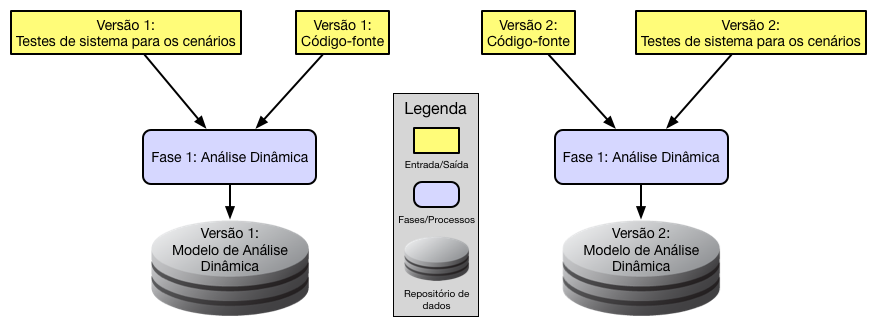
\includegraphics[scale=0.52]{Imagens/perfminer_fase_1.png}}
   \textsf{\caption[Fase 1 do \perfMinerName.]{Fase 1 do \perfMinerName.\label{fig:perfminer-fase1}}}
\end{figure}

O grafo é montado interceptando os métodos de entrada de cada cenário e instrumentando suas execuções, calculando o tempo de execução de cada nó, bem como informações sobre se o cenário falhou ou não. Esse grafo pode ser interpretado como uma estrutura em árvore onde cada nó é a execução de um método, onde os métodos de entrada representam os nós raiz \cite{Pinto2015}.

Duas informações são importantes nesse processo:
\begin{enumerate}[(i)]
   \item É fundamental que cada versão do sistema analisado possua testes automatizados para que o sistema seja executado. Caso o sistema não tenha testes automatizados, uma estratégia alternativa é utilizar ferramentas de teste de desempenho, como o \textit{JMeter} \cite{ApacheJMeter2016}, para submeter requisições que exercitem os cenários em um sistema web;
   \item Cada teste de sistema executado é considerado um cenário. Dessa forma, cada cenário analisado é representado na ferramenta com o seguinte nome: \textit{``Entry point for SimpleClassName.testMethodName''}.
\end{enumerate}

A ferramenta usa \textit{AspectJ} para definir um aspecto que instrumenta as execuções dos cenários, interceptando os métodos de entrada para montar o grafo de chamadas e calcular os tempos de execução dos cenários e dos seus métodos \cite{Pinto2015}.

De maneira sumária, o processo da figura \ref{fig:perfminer-fase1} se inicia com a execução dos testes de sistema, que são, então, interceptados pelo \textit{AspectJ} a fim de calcular seus tempos de execução. Após isso, o modelo de análise dinâmica resultante é persistido no banco de dados. Vale salientar que todo o processo dessa fase deve ser executado uma vez para cada versão do sistema a ser analisado. Dessa forma, serão gerados dois modelos de análise dinâmica que são utilizados para calcular os desvios de desempenho dos cenários e métodos na fase seguinte.

A análise dinâmica é executada no mesmo computador para todas as versões, nas mesmas condições e com todos os serviços não essenciais desabilitados (por exemplo: atualizações, antivírus, memória virtual). A suíte de testes para cada versão é executada, no mínimo, 10 vezes. Essa quantidade de execuções ajuda a ter medições de desempenho mais precisas em termos de tempo de execução.

\subsubsection{Fase 2: Análise de Desvio} \label{subsec:fase2}

A segunda fase é a análise de desvio, que consiste em realizar a comparação do modelo de análise dinâmica, extraído durante a fase de análise dinâmica, para cada uma das duas versões do sistema. Essa comparação revela os cenários e métodos que foram degradados ou otimizados durante a evolução. O artefato de saída desta fase é um relatório contendo os cenários e métodos degradados ou otimizados em termos de tempo de execução \cite{Pinto2015}. Esta fase pode ser vista na figura \ref{fig:perfminer-fase2} adiante.

\begin{figure}[!htb]
   \centering
   \frame{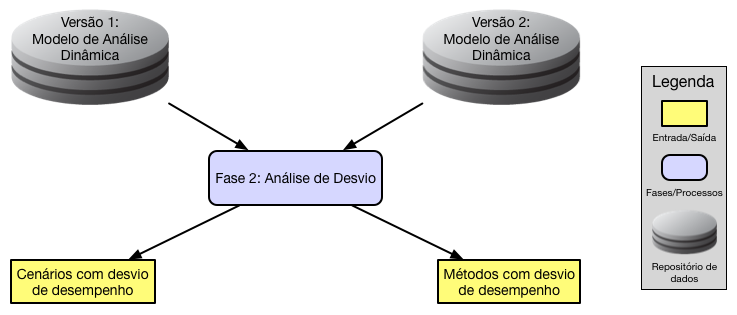
\includegraphics[scale=0.60]{Imagens/perfminer_fase_2.png}}
   \textsf{\caption[Fase 2 do \perfMinerName.]{Fase 2 do \perfMinerName.\label{fig:perfminer-fase2}}}
\end{figure}

Para realizar a comparação entre os tempos de execução, o \textit{\perfMinerName} pode utilizar duas estratégias: média aritmética e teste estatístico. A primeira compara a média do tempo de execução para cada método em ambas as versões. Se o valor da versão mais nova aumentou ou diminuiu mais do que um limiar configurado, é considerado que o método teve um desvio de desempenho. Já a segunda, usa um teste estatístico para observar se duas amostras independentes têm a mesma tendência. Neste caso, as amostras são formadas pelo conjunto dos valores dos tempos de execução para cada método comum em cada cenário \cite{Pinto2015}.

A estratégia de teste estatístico utilizado pela ferramenta é o Mann-Whitney U-Test \cite{Neuhauser2011}. Para esse teste, a ferramenta usa um valor padrão para o nível de significância (\textit{alpha}) de 0,05. Dado um método, se o \textit{p-value} calculado for igual ou menor do que o nível de significância, houve um desvio de desempenho para este método. Para os casos em que há o desvio, o tempo médio de execução é usado para determinar se houve uma degradação ou otimização. Embora, no geral, os desenvolvedores e arquitetos estejam interessados em degradações, a ferramenta também sinaliza as otimizações. Isso pode se tornar interessante, pois os desenvolvedores podem checar se algumas modificações esperadas realmente diminuíram o tempo de execução \cite{Pinto2015}.

\subsubsection{Fase 3: Mineração de Repositório} \label{subsec:fase3}

A última fase realiza a mineração nos repositórios de controle de versões e gerenciador de tarefas com o intuito de encontrar os \textit{commits} e tarefas que alteraram os métodos identificados na fase anterior. Para cada método detectado com desvio de desempenho (degradação ou otimização), esta fase recupera os commits do sistema de controle de versões. Se esse \textit{commit} alterou linhas dentro do método detectado, o número da respectiva tarefa é procurado na mensagem de \textit{commit}. O número da tarefa é usado para procurá-la no sistema de gerenciamento de tarefas em busca de informações extras, tais como o tipo da tarefa (defeito, melhoria, nova funcionalidade, etc) \cite{Pinto2015}. A figura \ref{fig:perfminer-fase3} ilustra essa fase.

\begin{figure}[!htb]
   \centering
   \frame{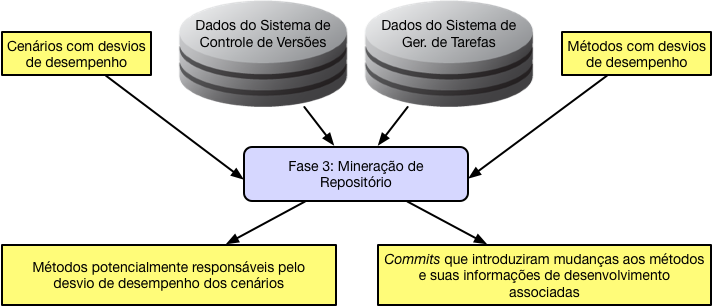
\includegraphics[scale=0.62]{Imagens/perfminer_fase_3.png}}
   \textsf{\caption[Fase 3 do \perfMinerName.]{Fase 3 do \perfMinerName.\label{fig:perfminer-fase3}}}
\end{figure}

É importante notar que os métodos identificados com desvios de desempenho nas fases anteriores, mas que não foram alterados durante a evolução, são também selecionados e armazenados, contudo, não estarão presentes no relatório final por, provavelmente, não representar causas reais do desvio de desempenho do cenário. Eles podem ter sido impactados por outros métodos na hierarquia de chamadas \cite{Pinto2015}.

A abordagem completa do \textit{\perfMinerName} pode ser vista na figura \ref{fig:perfminer-completo} adiante. Os artefatos de saída são usados como entradas para as fases seguintes, até a geração do relatório final. Os testes de sistemas em ambas as versões são considerados como os cenários para a análise e apenas os cenários e métodos comuns entre as versões são comparados.

\begin{figure}[!htb]
   \centering
   \frame{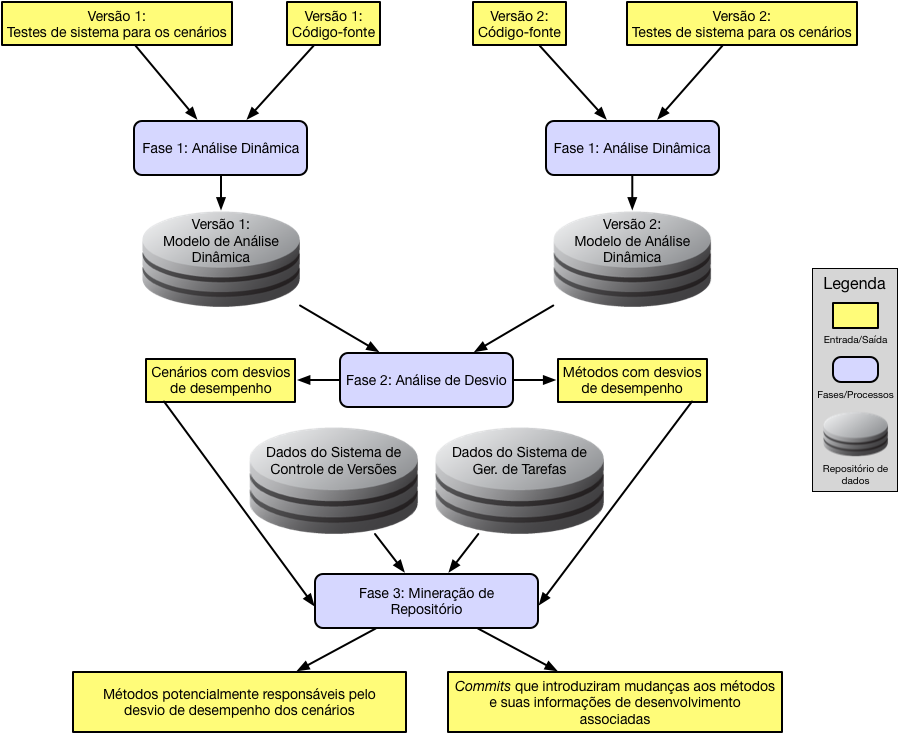
\includegraphics[scale=0.50]{Imagens/perfminer_completo.png}}
   \textsf{\caption[Abordagem completa do \perfMinerName.]{Abordagem completa do \perfMinerName.\label{fig:perfminer-completo}}}
\end{figure}

\begin{figure}[!htb]
   \centering
   \frame{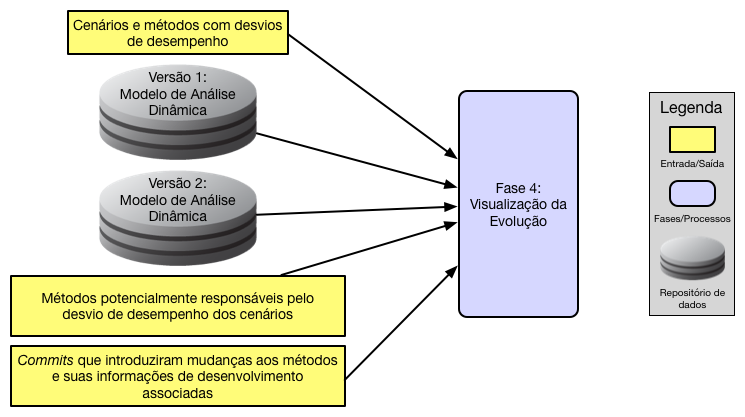
\includegraphics[scale=0.60]{Imagens/perfminer_fase_4.png}}
   \textsf{\caption[Fase 4 do \perfMinerName.]{Fase 4 do \perfMinerName.\label{fig:perfminer-fase4}}}
\end{figure}

As visualizações propostas como extensão da ferramenta utilizam os artefatos de saída gerados após a execução completa da abordagem, caracterizando assim mais uma fase da ferramenta: a Fase 4. Como ilustra a figura \ref{fig:perfminer-fase4} a seguir, os artefatos de saída utilizados pelas visualizações são: (i) os modelos de análise dinâmica de ambas as versões, (ii) os relatórios de cenários e métodos com desvios de desempenho, (iii) os métodos potencialmente responsáveis pelo desvio de desempenho dos cenários e (iv) os \textit{commits} que introduziram mudanças aos métodos, bem como suas informações de desenvolvimento associadas. Cada uma das visualizações implementadas utilizam total ou parcialmente os artefatos gerados nas fases anteriores, de acordo com o seu propósito.

\section{Visão Geral} \label{sec:visao-geral-architecture-qa-evolution}

A extensão ao \textit{\perfMinerName} foi implementada na forma de uma aplicação web, intitulada de \textit{Architecture QA Evolution}. O processamento do \textit{\perfMinerName} em suas fases 1, 2 e 3 não foi alterado, continuando \textit{standalone}. A escolha por esse tipo de aplicação se deu pelo fato de sua execução ocorrer em um ambiente distribuído, onde cada parte que compõe a aplicação está localizada em locais diferentes. Por exemplo, a interface com o usuário reside em sua estação de trabalho, ao passo que o servidor e o banco de dados estão localizados em outro computador.

Por ser web, os usuários da aplicação, como os desenvolvedores e arquitetos, podem utilizá-la sem a necessidade de instalar nenhum módulo nas suas estações de trabalho. Essa é uma importante característica da extensão à ferramenta, fazendo com que esta se diferencie das outras ferramentas mencionadas neste trabalho. A ideia é que distribuição e facilidade de acesso façam com que a equipe de desenvolvimento acompanhe mais adequadamente a evolução do atributo de qualidade de desempenho.

A implementação foi feita utilizando o \textit{framework} web Grails\footnote{\href{https://grails.org}{https://grails.org}}, banco de dados relacional PostgreSQL\footnote{\href{https://www.postgresql.org}{https://www.postgresql.org}} e o \textit{layout} das páginas foi elaborado lançando mão do \textit{framework front-end} Bootstrap\footnote{\href{http://getbootstrap.com}{http://getbootstrap.com}}. As visualizações foram geradas a partir de \textit{scripts} em JavaScript através da biblioteca JointJS\footnote{\href{https://www.jointjs.com}{https://www.jointjs.com}}. A estrutura das páginas web da ferramenta é dividida em três partes: canto superior, canto esquerdo e centro.

No canto superior situa-se uma barra de título, onde é apresentado o nome do sistema e o nome da página atual exibida. Na figura \ref{fig:pagina-inicial}, o nome do sistema é identificado como \texttt{\toolName} ao passo que o nome da página é \texttt{Analyzed Systems}.

Já no canto esquerdo é encontrada uma barra de menus contendo dois itens:
\begin{itemize}
   \item Nova análise (
\includegraphics[height=1.5em,valign=b]{Imagens/icon_new_analysis.png}): a partir deste item o usuário pode iniciar uma nova análise, que será descrita com maiores detalhes posteriormente;
   \item Sistemas analisados (
\includegraphics[height=1.5em,valign=b]{Imagens/icon_analyzed_systems.png}): é a página inicial mostrada na figura \ref{fig:pagina-inicial} explicada adiante.
\end{itemize}

Ao centro está a área principal da aplicação, onde são exibidas os conteúdos das páginas acessadas pelo usuário. Na página inicial exibida na figura \ref{fig:pagina-inicial}, pode ser verificada uma tabela contendo todos os sistemas analisados. Cada linha da tabela representa uma análise, onde são exibidas: a versão anterior (\textit{Version From}), versão posterior (\textit{Version To}), \textit{status} e ações (\textit{Actions}). No exemplo da figura, dois sistemas foram analisados pela ferramenta: o sistema \textit{System A} teve três análises e o sistema \textit{System B} teve quatro análises.

Dependendo do \textit{status} de cada análise, algumas ações pode ser tomadas. Caso o \textit{status} seja \texttt{COMPLETED}, o usuário pode navegar até a visualização de sumarização de cenários (
\includegraphics[height=1.5em,valign=b]{Imagens/visualizacao_1_icone.png}) ou apagar a análise (
\includegraphics[height=1.4em,valign=b]{Imagens/icon_delete_analysis.png}). Caso seja \texttt{ERROR}, a única ação que pode ser tomada é a de apagar a análise para que esta possa ser realizada novamente. Se o \textit{status} for \texttt{PENDING}, nenhuma ação pode ser efetuada uma vez que a análise ainda está em processamento.

\begin{figure}[htb]
   \centering
   \frame{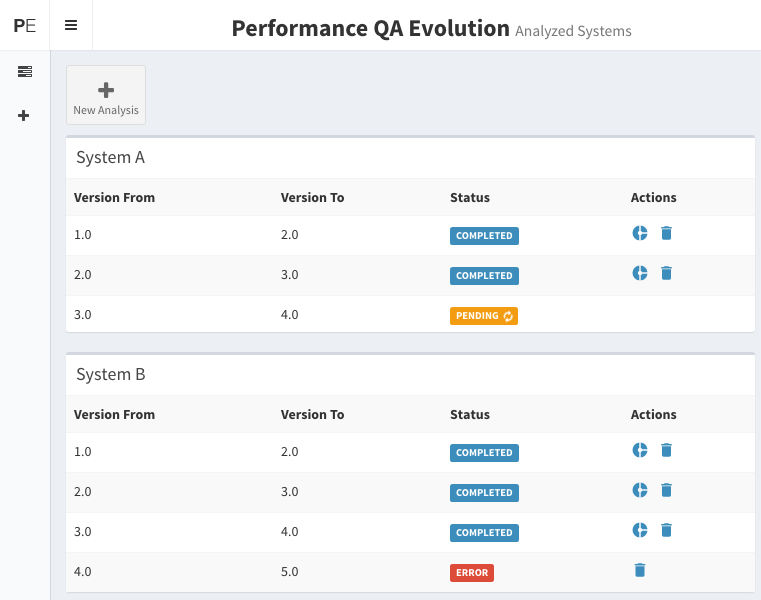
\includegraphics[scale=0.60]{Imagens/pagina_inicial.png}}
   \textsf{\caption[Página inicial da aplicação.]{Página inicial da aplicação.\label{fig:pagina-inicial}}}
\end{figure}

\subsection{Nova Análise} \label{subsec:new-analysis}

Para que o usuário da ferramenta obtenha acesso às visualizações é necessário que seja realizada uma análise dos artefatos gerados pelo \textit{\perfMinerName} onde, após o processamento, sejam gerados os dados responsáveis por supri-las.

A partir do menu de \texttt{Nova Análise} (
\includegraphics[height=1.5em,valign=b]{Imagens/icon_new_analysis.png}) ou do botão com o mesmo nome e ícone situado na página inicial (figura \ref{fig:pagina-inicial}), o usuário pode navegar até a página responsável por essa funcionalidade, exibida na figura \ref{fig:new-analysis}.

\begin{figure}[htb]
   \centering
   \frame{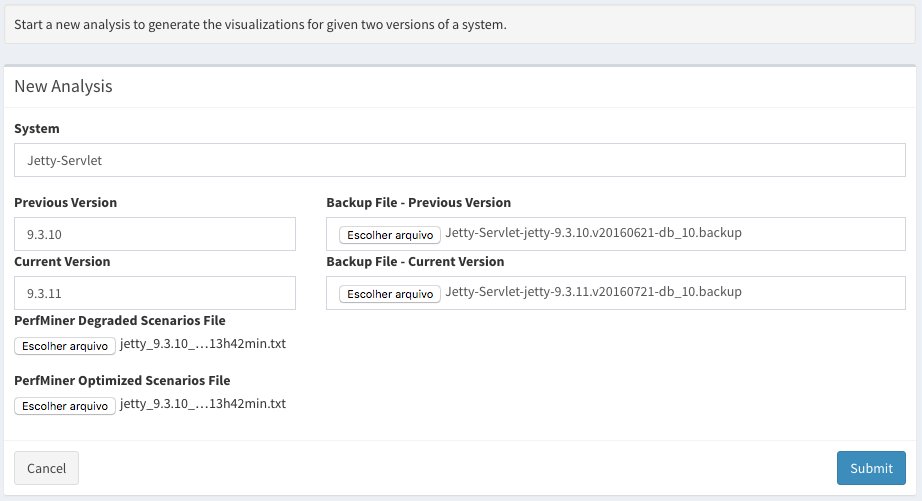
\includegraphics[scale=0.50]{Imagens/new_analysis.png}}
   \textsf{\caption[Página da funcionalidade de Nova Análise.]{Página da funcionalidade de Nova Análise.\label{fig:new-analysis}}}
\end{figure}

Nessa página, o usuário precisa informar os dados e arquivos necessários para que uma análise seja feita. No primeiro campo, o nome do sistema ao qual se deseja realizar a análise é informado. Após isso, é informada a versão anterior do sistema, no campo \texttt{Previous Version}, e o seu respectivo arquivo de \textit{backup} contendo os dados resultantes da análise do \textit{\perfMinerName}, no campo \texttt{Backup File - Previous Version}. Igualmente é feito para os campos \texttt{Current Version} e \texttt{Backup File - Current Version}, desta vez para a versão atual do sistema. Por fim, é necessário informar os arquivos contendo os cenários e métodos com desvio de desempenho, um para degradação de desempenho, no campo \texttt{\perfMinerName Degraded Scenarios File}, e outro para otimização de desempenho, no campo \texttt{\perfMinerName Optimized Scenarios File}.

\subsubsection{Funcionamento} \label{subsec:new-analysis-overview}

O funcionamento geral desta funcionalidade é ilustrado na figura \ref{fig:funcionamento-geral-nova-analise}. Vale salientar que esse processamento faz parte da fase 4 do \textit{\perfMinerName}, conforme exposto na figura \ref{fig:perfminer-fase4}. No primeiro passo desse processo (passo 1), o usuário realiza a requisição solicitando que uma nova análise seja realizada, de acordo com os parâmetros e arquivos informados na página da figura \ref{fig:new-analysis}.

\begin{figure}[!htb]
   \centering
   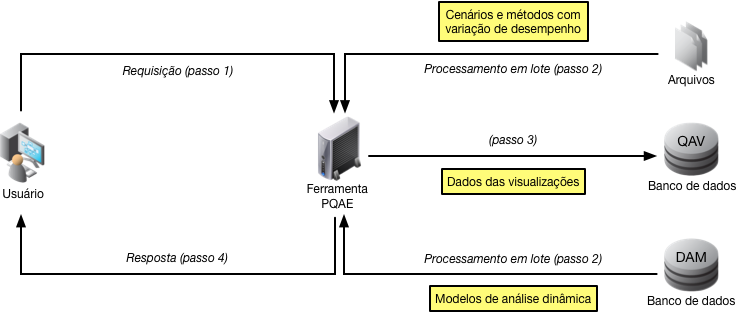
\includegraphics[scale=0.62]{Imagens/funcionamento_geral_nova_analise.png}
   \textsf{\caption[Funcionamento do processamento de uma nova análise.]{Funcionamento do processamento de uma nova análise.\label{fig:funcionamento-geral-nova-analise}}}
\end{figure}

Quando o servidor (Ferramenta PQAE) recebe essa requisição, inicia-se o processamento em lote (passo 2). Esse processamento recupera os arquivos contendo os cenários e métodos com desvio de desempenho que foram enviados pelo usuário, os arquivos de \textit{backups} referentes a versão anterior e atual a ser analisada. Os bancos de dados são restaurados e, então, os modelos de análise dinâmica para cada uma das versões são recuperadas desse banco de dados (identificado por \abrv[DAM -- \textit{Dynamic Analysis Model}]{DAM}– \textit{Dynamic Analysis Model}). De posse de todos esses dados, é realizado um processamento para determinar todos os dados que dão suporte às visualizações oferecidas pela ferramenta. Após isso, no passo 3, os dados resultantes são salvos em um banco de dados (identificado por \abrv[QAV -- \textit{Quality Attribute Visualization}]{QAV}– \textit{Quality Attribute Visualization}). Ao final, o usuário recebe a resposta de que o processamento requisitado foi efetuado com sucesso, no passo 4.

Detalhadamente, no processamento em lote, iniciado no passo 2, os arquivos de saída do \textit{\perfMinerName} contendo informações sobre os cenários e métodos com desvio de desempenho são lidos e os modelos de análise dinâmica de ambas as versões são recuperados do banco de dados DAM. A partir de então, os dados para cada visualização começam a ser processados. Os passos 2 e 3 da figura \ref{fig:funcionamento-geral-nova-analise} são detalhados no diagrama de atividades da figura \ref{fig:nova-analise-passos-2-3}.

De posse desses artefatos, os nós do grafo de chamadas são recuperados e a partir deles são determinados os métodos que foram adicionados ou removidos comparando os nós da versão atual com os da anterior. Depois disso, a partir dos métodos indicados pelos arquivos de saída do \textit{\perfMinerName}, são determinados os nós com desvios de desempenho, seja degradação ou otimização.

Na ferramenta, os nós identificados como adicionados, removidos e com desvio de desempenho são candidatos a serem exibidos. Optou-se por apresentar apenas os nós com desvio, nós adicionados, removidos e poucos nós sem desvio de desempenho, mas que ajudam a tornar o grafo legível, de modo que poucos nós são renderizados no navegador do usuário. Essa decisão levou em consideração a quantidade de nós de um cenário, que pode passar dos milhares, o desempenho da própria aplicação web e um possível ganho no entendimento da visualização do grafo de chamadas por parte do usuário.

\begin{figure}[!htb]
   \centering
   \frame{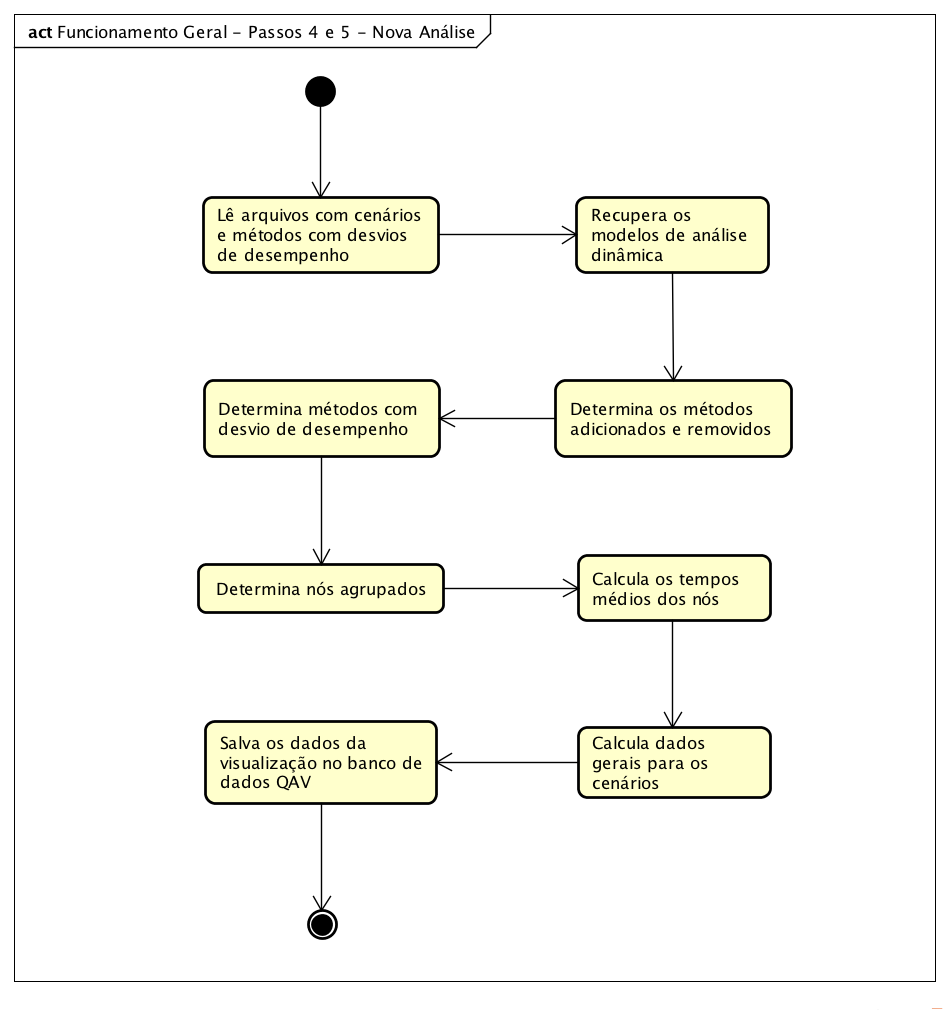
\includegraphics[scale=0.45]{Imagens/funcionamento_geral_nova_analise_diagrama_atividades.png}}
   \textsf{\caption[Passos 2 e 3 da realização de uma nova análise.]{Passos 2 e 3 da realização de uma nova análise.\label{fig:nova-analise-passos-2-3}}}
\end{figure}

Após determinar os nós com desvios de desempenho, são criados nós de agrupamento para representar os que não serão exibidos na visualização. Depois disso, os tempos médios dos nós a serem exibidos são calculados, levando em consideração todas as ocorrências do método no cenário.

Para a visualização da sumarização de cenários, os dados gerais de todos os cenários são calculados e, juntamente com os dados da visualização do grafo de chamadas calculados anteriormente, são salvos no banco de dados QAV no passo 3, marcando o fim do processo.

É importante frisar que o processamento em lote é executado apenas uma vez para duas versões de um sistema, sendo necessário para gerar os dados que possibilitam aos usuários um rápido tempo de resposta na requisição das visualizações.

\FloatBarrier

\subsubsection{Bancos de Dados} \label{subsec:databases}

Os bancos de dados DAM e QAV mencionados anteriormente têm funções distintas. O DAM é utilizado pelo \textit{\perfMinerName} para armazenar os dados coletados na análise dinâmica. Já o QAV é próprio da ferramenta \textit{\toolName} e armazena os dados que dão suporte às visualizações, funcionando também como um \textit{cache}, minimizando o tempo de resposta do servidor para o usuário.

\paragraph{DAM - \textit{Dynamic Analysis Model}} \label{par:estrutura-dados-dam}

O resultado do processamento da fase 1 do \textit{\perfMinerName} gera um modelo de análise dinâmica que contém informações sobre os \textit{traces} de execução do sistema, como mencionado na subseção \ref{subsec:fase1}. Esse modelo é persistido no banco de dados DAM, sendo usado, posteriormente, na extensão proposta por este trabalho para gerar as visualizações. A figura \ref{fig:perfminer-class-diagram} a seguir mostra o diagrama de classes parcial desse modelo.

\begin{figure}[!htb]
   \centering
   \frame{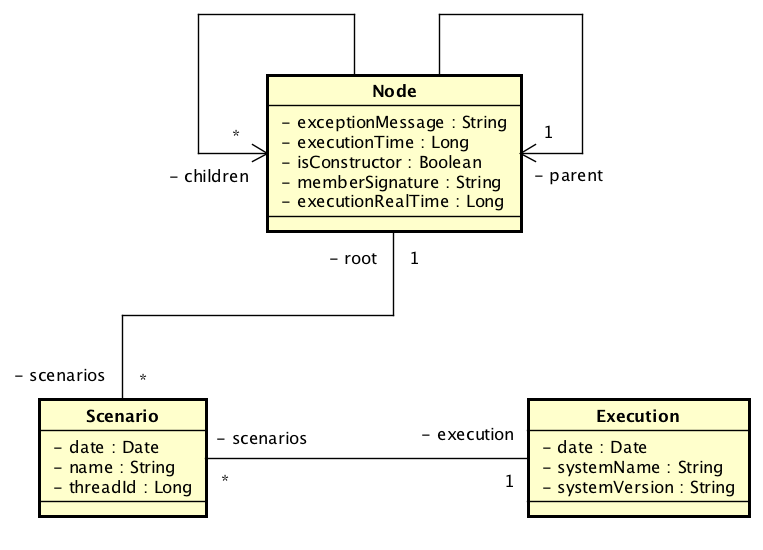
\includegraphics[scale=0.50]{Imagens/perf_miner_class_diagram.png}}
   \textsf{\caption[Diagrama de classes parcial do \textit{\perfMinerName}.]{Diagrama de classes parcial do \textit{\perfMinerName}.\label{fig:perfminer-class-diagram}}}
\end{figure}

A classe \texttt{Execution} representa uma execução específica do \textit{\perfMinerName} para um sistema. Possui atributos que indicam o nome do sistema, a versão e a data que a análise foi iniciada. Já a classe \texttt{Scenario} é o modelo para cada cenário executado. Os cenários têm um nome, uma data que indica quando foi analisado, o \texttt{id} da \textit{thread} que o executou, o contexto para representar requisições web (em caso de sistemas web) e o nó raiz.

A classe \texttt{Node} representa todo membro (método ou construtor) executado dentro de um cenário em particular. Essa classe possui atributos para indicar a assinatura do método ou construtor, uma mensagem se alguma exceção acontecer durante a execução, o tempo de execução total do membro, o tempo de execução do próprio membro, uma propriedade booleana que indica se o nó representa ou não um construtor e dois autorrelacionamentos: um para indicar o nó pai e outro para indicar os nós filhos. Uma atenção especial merece ser dada aos dois tempos de execução: a propriedade \texttt{executionRealTime} indica o tempo de execução do próprio método ou construtor, sem considerar os tempos de execução dos nós filhos. Já a propriedade \texttt{executionTime} representa o tempo total de execução do membro, considerando os tempos dos membros filhos.

\paragraph{QAV - \textit{Quality Attribute Visualization}} \label{par:estrutura-dados-qav}

A ferramenta faz uso de outro banco de dados além do DAM: o QAV. Essa base de dados é responsável por armazenar os dados que darão suporte às visualizações. A figura \ref{fig:archvis-class-diagram} a seguir mostra o diagrama de classes para esse modelo.

\begin{figure}[!htb]
   \centering
   \frame{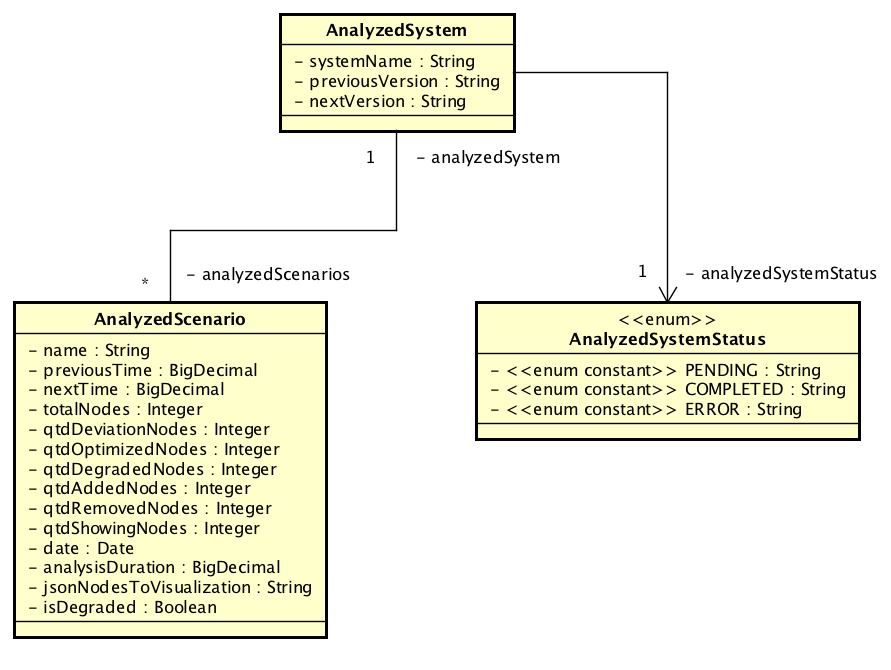
\includegraphics[scale=0.50]{Imagens/arch_vis_class_diagram.png}}
   \textsf{\caption[Diagrama de classes da extensão proposta.]{Diagrama de classes da extensão proposta.\label{fig:archvis-class-diagram}}}
\end{figure}

A classe \texttt{AnalyzedSystem} representa uma análise para dado sistema, em determinadas versões. Possui propriedades para o nome do sistema, versão anterior e versão posterior. Cada análise possui um \textit{status}, definido pela propriedade \texttt{analyzedSystemStatus} dessa classe, do tipo \texttt{AnalyzedSystemStatus}. Essa propriedade pode assumir um dos três valores a seguir: \texttt{PENDING} (análise em andamento), \texttt{COMPETED} (análise finalizada), \texttt{ERROR} (análise com erro - necessário novo processamento).

A classe \texttt{AnalyzedScenario} reflete cada cenário analisado de determinadas versões. Possui propriedades para o nome do cenário, tempos de execução na versão anterior e posterior, total de nós do grafo de chamadas, quantidade de nós otimizados, degradados, adicionados, removidos e exibidos no grafo, data e hora do processamento da análise, um atributo booleano que indica se o cenário é de otimização ou degradação e um atributo que armazena o JSON que dá suporte à visualização do grafo de chamadas. Embora existam atributos que armazenem dados referentes a visualização do grafo de chamadas, essas classes foram modeladas de modo a dar suporte a todas as visualizações propostas neste trabalho.

\section{Visualização da Sumarização de Cenários} \label{sec:visualizacao1}

A Sumarização dos Cenários permite ao usuário obter uma visualização dos cenários com desvios de desempenho entre duas versões do sistema. Para essa visualização foi utilizada uma variação do gráfico de rosca, que por sua vez é uma derivação do de pizza. O gráfico de pizza é considerado um gráfico de informação simples cujo principal objetivo é mostrar a relação de uma parte com o todo \cite{Spence2005}. No contexto da visualização apresentada, o todo se configura como sendo todos os cenários com desvios de desempenho para as versões analisadas, e as partes são cada cenário com suas características.

A algura, a largura e a cor de uma fatia do grático são as características visuais que possuem significado nessa visualização:

\begin{itemize}
   \item \textit{Largura}: a largura de uma fatia do gráfico indica a porcentagem de desvio de desempenho do cenário na versão atual relacionado com a versão anterior. Quanto mais larga a fatia, maior foi o desvio de desempenho. De maneira contrária, quanto mais fina a fatia, menor o desvio;
   \item \textit{Altura}: a altura da fatia indica o tempo de execução do cenário na versão atual. Quanto mais alta a área preenchida, maior o tempo de execução. De maneira contrária, quanto mais baixa, menor o tempo de execução;
   \item \textit{Cor}: cada fatia do gráfico possui uma cor que indica se houve degradação ou otimização no desempenho do cenário. A cor marrom claro indica que o cenário foi degradado, ao passo que a cor verde indica que ele foi otimizado em relação a versão anterior.
\end{itemize}

A figura \ref{fig:visualizacao-1-visal-geral} exibe uma visão geral desta visualização. Na parte superior, é possível notar 5 blocos com as seguintes informações: nome do sistema, versões analisadas (anterior e atual), quantidade de cenários com desvios de desempenho, quantidade de cenários com degradação e quantidade de cenários com otimização. Na parte central, encontra-se o gráfico. Nele, existem 5 divisões, onde cada uma delas representa um cenário e possui largura, altura e cor. Na parte superior direita, há uma legenda explicativa sobre altura, a largura e as cores das fatias.

\begin{figure}[htb]
   \centering
   \frame{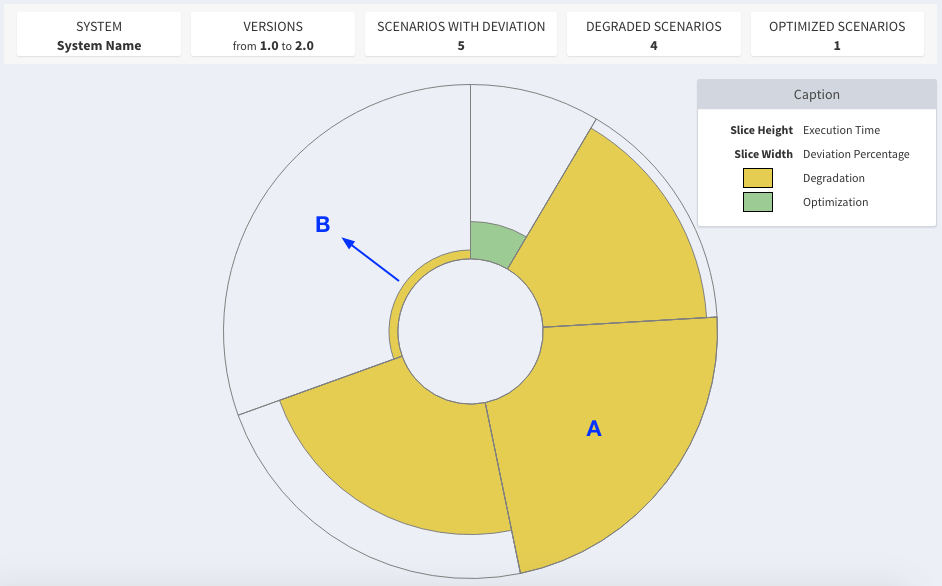
\includegraphics[scale=0.48]{Imagens/sumarizacao_cenarios_visao_geral.png}}
   \textsf{\caption[Visão geral da Sumarização de Cenários.]{Visão geral da Sumarização de Cenários.\label{fig:visualizacao-1-visal-geral}}}
\end{figure}

A partir do gráfico da figura \ref{fig:visualizacao-1-visal-geral}, podem ser vistos 4 cenários com degradação de desempenho e 1 cenário com otimização. Dos cenários com degradação, 3 deles possuem os maiores tempos de execução perante o restante (altura da fatia). A respeito do cenário com otimização, pode-se notar que possui baixo tempo de execução com relação aos demais (altura da fatia) e tem o menor desvio de desempenho com relação à versão anterior analisada (largura da fatia). O cenário indicado pela letra \texttt{A} foi o cenário com maior tempo de execução dentre os analisados, como evidencia a altura da fatia. Já o cenário indicado pela letra \texttt{B} foi o que possuiu a maior variação de desempenho, destacado pela largura da fatia.

\subsection{Interação} \label{subsec:visualizacao1-interacao}

O gráfico desta visualização é passível de ações do usuário, a fim de (i) obter maiores informações sobre determinado cenário ou (ii) avançar para a visualização do grafo de chamadas, descrita mais adiante neste trabalho. Para a primeira ação, o usuário deve posicionar o ponteiro do \textit{mouse} sobre uma das fatias do gráfico e então um \textit{tooltip} é apresentado, como pode ser visto na figura \ref{fig:visualizacao-1-tooltip}.

\begin{figure}[htb]
   \centering
   \frame{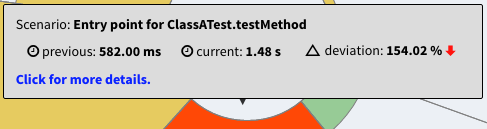
\includegraphics[scale=0.65]{Imagens/sumarizacao_cenarios_tooltip.png}}
   \textsf{\caption[\textit{Tooltip} com maiores informações sobre determinado cenário.]{\textit{Tooltip} com maiores informações sobre determinado cenário.\label{fig:visualizacao-1-tooltip}}}
\end{figure}

No \textit{tooltip} mostrado, é possível verificar o nome do cenário: \texttt{Entry point for ClassA\\Test.testMethod}; o seu tempo de execução na versão anterior: \texttt{582,00 milissegundos}; o tempo de execução na versão atual: \texttt{1,48 segundos}; e a porcentagem de desvio do tempo de execução da versão atual em relação a versão anterior: uma degradação de \texttt{154,02\%}. É possível concluir que houve uma degradação através da seta vermelha para baixo. Em caso de seta verde para cima, significa que houve uma otimização de desempenho. Ao clicar em uma das fatias do gráfico, o usuário será levado para a visualização do grafo de chamadas.

\subsection{Funcionamento} \label{subsec:sumarizacao-cenarios-funcionamento}

As visualizações apresentadas neste trabalho seguem o mesmo padrão, apresentado na figura \ref{fig:funcionamento-geral-visualizacoes}. Os usuários somente terão acesso às visualizações quando uma análise para a versão desejada já tiver sido processada.

\begin{figure}[!htb]
   \centering
   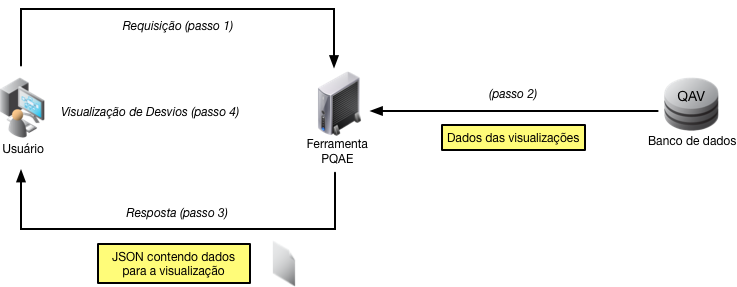
\includegraphics[scale=0.62]{Imagens/funcionamento_geral_visualizacoes.png}
   \textsf{\caption[Funcionamento geral das visualizações.]{Funcionamento geral das visualizações.\label{fig:funcionamento-geral-visualizacoes}}}
\end{figure}

A partir da listagem das análises realizadas na página inicial da aplicação, exibida na figura \ref{fig:pagina-inicial}, o usuário pode clicar no ícone desta visualização (
\includegraphics[height=1.5em,valign=b]{Imagens/visualizacao_1_icone.png}) para acessá-la. Ao clicar, é realizada uma requisição para a aplicação, solicitando acesso à visualização de sumarização de cenários (passo 1). O servidor (Ferramenta PQAE) recebe essa requisição e, a partir dos dados referentes ao sistema e versões desejadas, recupera do banco de dados QAV (passo 2) os dados necessários para a visualização. Após isso, é retornado para o \textit{browser} do usuário um arquivo em formato \abrv[JSON -- \textit{JavaScript Object Notation}]{JSON}(\textit{JavaScript Object Notation}) contendo os dados recuperados (passo 3). O \textit{browser}, por fim, recebe, interpreta esse arquivo e monta a visualização com as devidas informações para que a renderização seja feita com sucesso (passo 4).

O processamento realizado quando o usuário recebe a resposta está exposto na figura \ref{fig:sumarizacao-cenarios-passo-4}. Ao receber o arquivo JSON do servidor, o navegador define a área de desenho que abrigará o gráfico baseado na altura e largura do monitor do usuário. Após isso, é determinado, dentre os cenários indicados pela análise, qual o que possuiu o maior tempo de execução. Esse tempo é utilizado para estabelecer o limite das fatias do gráfico. Isto posto, pelo menos um cenário preencherá por completo uma das fatias do gráfico. Na sequência, a cor, largura e altura, além dos dados do \textit{tooltip} de cada fatia são determinadas baseadas nos dados dos respectivos cenários. Por fim, o gráfico é criado e renderizado.

\begin{figure}[htb]
   \centering
   \frame{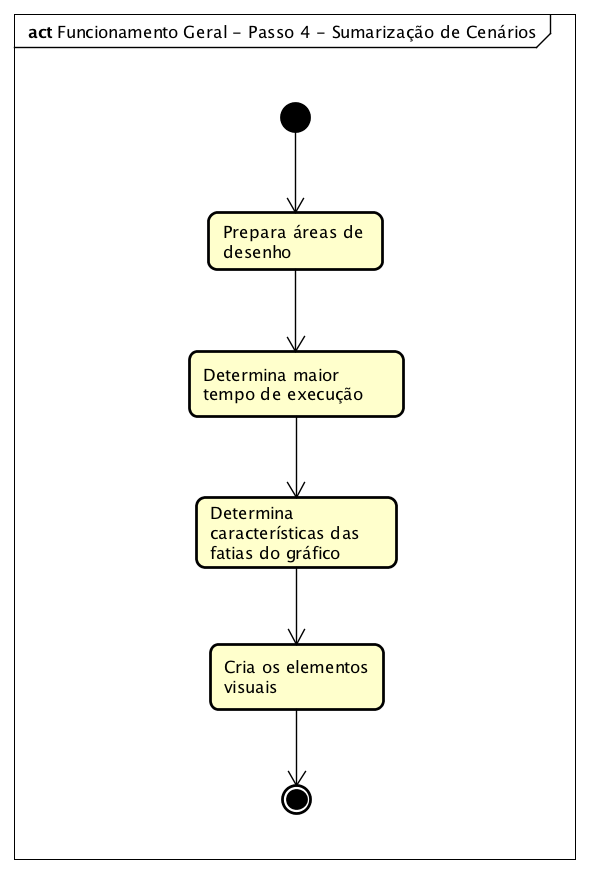
\includegraphics[scale=0.45]{Imagens/sumarizacao_cenarios_passo_4.png}}
   \textsf{\caption[Detalhamento do passo 4 da figura \ref{fig:funcionamento-geral-visualizacoes}, na Sumarização de Cenários.]{Detalhamento do passo 4 da figura \ref{fig:funcionamento-geral-visualizacoes}, na Sumarização de Cenários.\label{fig:sumarizacao-cenarios-passo-4}}}
\end{figure}

\section{Visualização do Grafo de Chamadas} \label{sec:visualizacao2}

Esta visualização tem o objetivo de mostrar, para dadas duas versões de um sistema, os métodos que potencialmente causaram o desvio de desempenho para um determinado cenário. Esses métodos são exibidos em um grafo direcionado de chamadas com propriedades visuais que destacam quais dos métodos mostrados tiveram desvios de desempenho.

Os grafos podem ser utilizados quando os dados a serem representados são estruturados, ou seja, quando existe uma relação inerente entre os elementos de dados a serem visualizados \cite{Herman2000}. Há uma vasta quantidade de áreas onde os grafos podem ser aplicados, por exemplo: hierarquia de arquivos em formato de árvore, mapas de sites, mapas moleculares e genéticos, diagramas de fluxos de dados, entre outros \cite{Herman2000}.

Nesse sentido, em uma chamada de métodos é evidente a relação entre eles, uma vez que os objetos, em um sistema orientado a objetos, trocam mensagens entre si através da invocação dos métodos. O grafo é exibido utilizando o \textit{layout} em árvore, onde os nós filhos estão dispostos abaixo dos nós ancestrais, e a direção dos nós é \textit{top-down}. Um exemplo do grafo é exibido na figura \ref{fig:grafo-chamadas-exemplo}. Nesta seção serão detalhadas as suas propriedades visuais, o seu funcionamento básico, além de descrever a seção de Sumário e Histórico desta visualização.

\begin{figure}[htb]
   \centering
   \frame{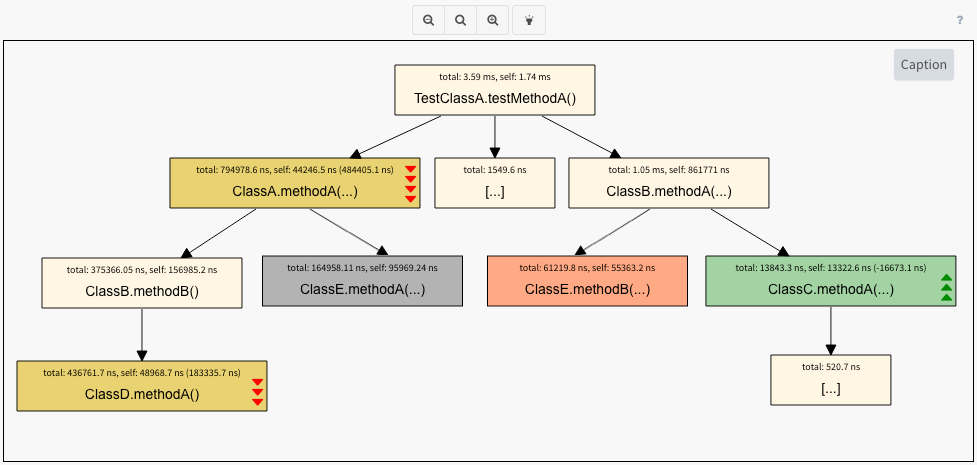
\includegraphics[scale=0.46]{Imagens/grafo_chamadas_exemplo.png}}
   \textsf{\caption[Exemplo do grafo de chamadas.]{Exemplo do grafo de chamadas.\label{fig:grafo-chamadas-exemplo}}}
\end{figure}

\subsection{Sumário} \label{subsubsec:visualizacao2-sumario}

A seção Sumário está disponível acima da seção do Grafo de Chamadas e o seu intuito é trazer outras informações à visualização visando auxiliar os usuários na contextualização do cenário exibido.

\begin{figure}[htb]
   \centering
   \frame{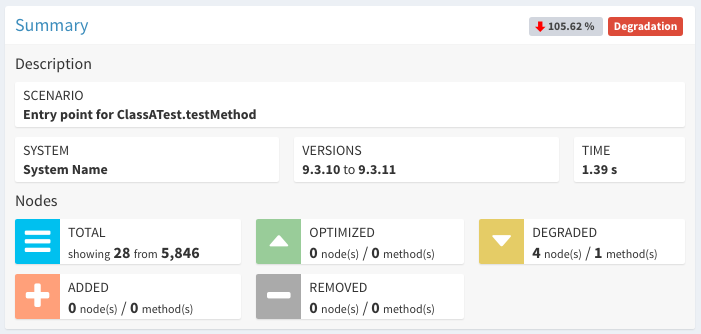
\includegraphics[scale=0.65]{Imagens/grafo_chamadas_sumario.png}}
   \textsf{\caption[Seção de sumário do grafo de chamadas.]{Seção de sumário do grafo de chamadas.\label{fig:grafo-chamadas-sumario}}}
\end{figure}

Na figura \ref{fig:grafo-chamadas-sumario}, é mostrada uma visão geral sobre determinado cenário sendo exibido na visualização. Para a seção \textit{Description}, as informações exibidas são:
\begin{itemize}
   \item \textit{Scenario}: exibe o nome do cenário analisado;
   \item \textit{System}: nome do sistema analisado;
   \item \textit{Versions}: versões do sistema que foram analisadas. É mostrado no formato \textit{<versionA>} to \textit{<versionB>}. Espera-se que a versão B, neste caso, seja posterior a versão A;
   \item \textit{Time}: mostra o tempo de execução do cenário na versão mais recente. A diferença de tempo entre as duas versões vai guiar o que será exibido na barra de títulos da figura. No exemplo mostrado, o tempo na última versão degradou com relação ao tempo na versão anterior, sendo exibido, no canto superior direito, a porcentagem da degradação (\texttt{105,62\%}) acompanhada de uma seta vermelha para baixo e um rótulo em vermelho marcando o cenário como degradado (\textit{degradation}). Caso o tempo do cenário seja otimizado, é exibida uma seta verde para cima ao lado da porcentagem da variação, além de um rótulo verde marcando o cenário como otimizado (\textit{optimization}).
\end{itemize}

Para a seção \textit{Nodes}, as informações são as seguintes:
\begin{itemize}
   \item \textit{Total}: mostra o número de nós que estão sendo mostrados no grafo de chamadas e total de nós do cenário. Vale salientar que cada nó representa um método executado durante a hierarquia de chamadas do cenário. Pode acontecer de nós diferentes representarem o mesmo método. Isso pode acontecer porque o mesmo método pode ter hierarquias de chamadas diferentes;
   \item \textit{Optimized}: exibe o número de nós e métodos que tiveram otimização de desempenho. Para que um determinado nó seja considerado com otimização de desempenho, ele (i) tem que estar presente nas duas versões analisadas e (ii) o tempo de execução na versão posterior tem que ter sido menor do que na versão anterior;
   \item \textit{Degraded}: exibe o número de nós e métodos que tiveram degradação de desempenho. Para que um determinado nó seja considerado com degradação de desempenho, ele (i) tem que estar presente nas duas versões analisadas e (ii) o tempo de execução na versão posterior tem que ter sido maior do que na versão anterior;
   \item \textit{Added}: apresenta o número de nós e métodos que foram adicionados da versão anterior para a posterior. Ou seja, são os métodos que não existiam na execução do cenário para a versão anterior e passaram a existir na execução da versão posterior. O número de métodos pode ser menor do que o número de nós, uma vez que nós diferentes podem representar o mesmo método;
   \item \textit{Removed}: o contrário do conceito anterior. São apresentados os nós e métodos que foram removidos da versão anterior para a posterior.
\end{itemize}

Para as informações sobre os nós otimizados, degradados, adicionados e removidos, o número de métodos pode ser menor do que o número de nós, uma vez que nós diferentes podem representar o mesmo método se eles estiverem em hierarquias de chamadas diferentes.

\subsection{Histórico} \label{subsubsec:visualizacao2-historico}

A segunda parte da visualização do Grafo de Chamadas apresenta o histórico da evolução do desempenho, em termos de tempo de execução, de determinado cenário. A exibição do histórico é em formato de um gráfico de linha, onde no eixo X são apresentadas as dez últimas versões analisadas em que o cenário esteve presente e no eixo Y é mostrado o tempo de execução. A figura \ref{fig:grafo-chamadas-historico} adiante mostra um exemplo desse gráfico.

\begin{figure}[!htb]
   \centering
   \frame{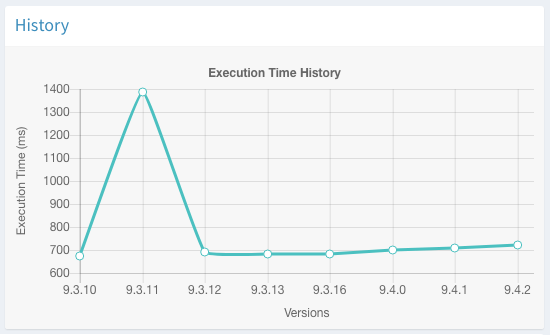
\includegraphics[scale=0.65]{Imagens/grafo_chamadas_historico.png}}
   \textsf{\caption[Seção de histórico do grafo de chamadas.]{Seção de histórico do grafo de chamadas.\label{fig:grafo-chamadas-historico}}}
\end{figure}

Na figura, pode-se concluir que o cenário em questão esteve presente nas versões \texttt{9.3.10}, \texttt{9.3.11}, \texttt{9.3.12}, \texttt{9.3.13}, \texttt{9.3.16}, \texttt{9.4.0}, \texttt{9.4.1} e \texttt{9.4.2}. Entre as versões \texttt{9.3.10} e \texttt{9.3.11}, nota-se uma forte degradação, praticamente duplicando o seu tempo de execução. Por outro lado, da versão \texttt{9.3.11} para a \texttt{9.3.12}, houve uma otimização importante, o que resultou em um tempo de execução próximo ao da versão \texttt{9.3.10}. Da \texttt{9.3.12} a \texttt{9.4.2} pequenas degradações são notadas no desempenho do cenário.

\FloatBarrier % evite que as figuras da subsecao anterior invadam a secao seguinte

\subsection{Grafo de Chamadas} \label{subsubsec:visualizacao2-grafo-chamadas}

A terceira e última parte da visualização é o grafo de chamadas propriamente dito. Esse grafo, como mencionado, é composto de nós e arestas direcionadas que expõem os caminhos das chamadas dos métodos para o cenário analisado. Os nós, representados por caixas, possuem algumas características visuais, apresentadas adiante.

\subsubsection{Nó sem desvio} \label{subsec:no-sem-desvio}

\begin{figure}[htb]
   \centering
   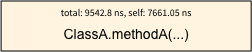
\includegraphics[scale=0.65]{Imagens/no_sem_desvio.png}
   \textsf{\caption[Nó que representa um método sem desvio de desempenho.]{Nó que representa um método sem desvio de desempenho.\label{fig:no-sem-desvio}}}
\end{figure}

O primeiro e mais básico tipo de nó é o que representa um método que não teve desvios de desempenho para o cenário e versões analisadas, apresentado na figura \ref{fig:no-sem-desvio}. As características desse nó são:\tabularnewline
\begin{itemize}
   \item \textit{Cor}: esta é a principal característica que diferencia os nós uns dos outros. No caso deste nó, a cor é marrom claro;
   \item \textit{Nome do nó}: posicionado ao centro, são mostrados o nome da classe e o nome do método executado, no formato \texttt{ClassName.methodName()}. Para otimizar e evitar a exibição de grande quantidade de texto, o nome do pacote e os parâmetros do método foram ocultados, sendo estes, quando houver, representados por três pontos (...). Essa definição serve para todos os tipos de nós dessa visualização;
   \item \textit{Tempos de execução}: localizados no canto superior do nó, são apresentados dois tempos de execução: à esquerda, o tempo total do nó, que representa a soma dos tempos de execução dos nós filhos com o tempo do próprio nó. No exemplo da figura, o tempo total foi de \texttt{9.542,8} nanossegundos; e à direita, o tempo do próprio nó, desconsiderando o tempo dos nós filhos. Na figura, o tempo foi de \texttt{7.661,05} nanossegundos.
   %\item \textit{Detalhes}: no canto superior esquerdo é exibido um ícone onde, ao passar o cursor do \textit{mouse}, o usuário pode obter mais informações sobre o nó. No caso de um nó sem desvio de desempenho, as informações exibidas nesta seção são o nome do pacote e os parâmetros do método, se houver. A figura \ref{fig:detalhes-no-sem-desvio} a seguir mostra essa seção.
\end{itemize}

% \begin{figure}[htb]
%    \centering
%    \frame{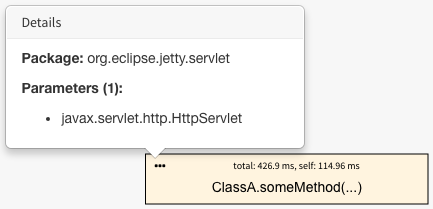
\includegraphics[scale=0.65]{Imagens/detalhes_no_sem_desvio.png}}
%    \textsf{\caption[Seção de detalhes do nó sem desvio de desempenho.]{Seção de detalhes do nó sem desvio de desempenho.\label{fig:detalhes-no-sem-desvio}}}
% \end{figure}

\subsubsection{Nó degradado} \label{subsec:no-degradado}

 A visualização também é capaz de apontar se determinado nó teve o seu desempenho degradado com relação à versão anterior. A figura \ref{fig:no-degradado} apresenta um nó degradado:

\begin{figure}[htb]
   \centering
   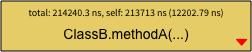
\includegraphics[scale=0.65]{Imagens/no_degradado.png}
   \textsf{\caption[Nó que representa um método com degradação de desempenho.]{Nó que representa um método com degradação de desempenho.\label{fig:no-degradado}}}
\end{figure}

As características visuais deste nó são bem semelhantes às apresentadas para os nós otimizados:
\begin{itemize}
   \item \textit{Cor}: os nós que degradaram o desempenho são mostrados em laranja amarelo;
   \item \textit{Tempos de execução}: além dos tempos total e do próprio nó, um nó com desvio de desempenho, seja otimização ou degradação, apresenta a diferença entre os tempos de execução da versão anterior para a posterior entre parênteses, no canto superior direito. No exemplo da figura, o nó degradou o seu tempo em \texttt{12.202,79} nanossegundos;
   \item \textit{Setas}: no canto inferior direito são mostradas setas indicativas de quão forte ou fraca foi a variação de desempenho. No caso de nós com degradação, são exibidas setas vermelhas apontadas para baixo, onde cada uma delas representa 25\% de desvio do tempo com relação à versão anterior. Sendo assim, uma única seta representa um desvio de 0 a 25\%, duas setas de 25\% a 50\%, três setas de 50\% a 75\% e quatro setas de 75\% ou superior. No exemplo apresentado na figura \ref{fig:no-degradado}, a degradação se deu entre 0 e 25\% do tempo de exeução em relação ao desempenho anterior.
   %\item \textit{Detalhes}: esta seção possui as mesmas informações dos nós relatados até aqui, como podem ser vistas na figura \ref{fig:detalhes-no-degradado} a seguir.
\end{itemize}

% \begin{figure}[htb]
%    \centering
%    \frame{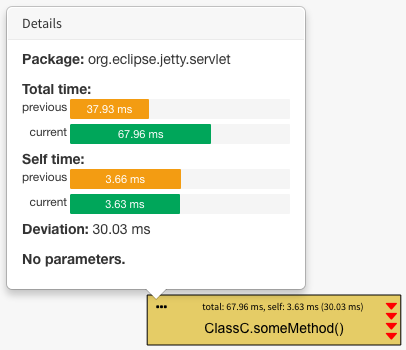
\includegraphics[scale=0.65]{Imagens/detalhes_no_degradado.png}}
%    \textsf{\caption[Seção de detalhes do nó com degradação de desempenho.]{Seção de detalhes do nó com degradação de desempenho.\label{fig:detalhes-no-degradado}}}
% \end{figure}

\subsubsection{Nó otimizado} \label{subsec:no-otimizado}

Quando um cenário possui nós que otimizaram o seu desempenho em relação a versão anterior, outros elementos visuais são acrescidos à visualização. A figura \ref{fig:no-otimizado} a seguir apresenta um nó otimizado:

\begin{figure}[htb]
   \centering
   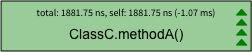
\includegraphics[scale=0.65]{Imagens/no_otimizado.png}
   \textsf{\caption[Nó que representa um método com otimização de desempenho.]{Nó que representa um método com otimização de desempenho.\label{fig:no-otimizado}}}
\end{figure}

As características visuais deste nó, além das comentadas anteriormente, são:
\begin{itemize}
   \item \textit{Cor}: os nós que otimizaram o atributo de qualidade desempenho são mostrados em um tom de verde;
   \item \textit{Tempos de execução}: também são exibidos os tempos de execução total, do próprio nó e o desvio de desempenho. No exemplo, o nó otimizou o tempo em \texttt{1,07} milissegundos;
   \item \textit{Setas}: as setas indicativas de variação de desempenho para nós de otimização são apontadas para cima, de cor verde. No exemplo, a otimização se deu em mais de 75\% do desempenho em relação à versão anteiror.
   %\item \textit{Detalhes}: esta seção para os nós com otimização de desempenho possui informações diferentes das relatadas anteriormente, como podem ser vistas na figura \ref{fig:detalhes-no-otimizado}. Além das informações sobre o pacote e os parâmetros, também são apresentadas sobre os tempos de execução da versão anterior e posterior, além da variação de tempo.
\end{itemize}

%\begin{figure}[htb]
%    \centering
%    \frame{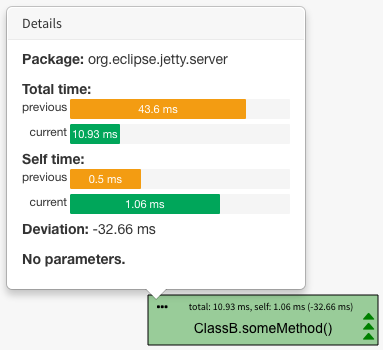
\includegraphics[scale=0.65]{Imagens/detalhes_no_otimizado.png}}
%    \textsf{\caption[Seção de detalhes do nó com otimização de desempenho.]{Seção de detalhes do nó com otimização de desempenho.\label{fig:detalhes-no-otimizado}}}
% \end{figure}

\subsubsection{Nó adicionado} \label{subsec:no-adicionado}

Um cenário pode apresentar, para diferentes versões, nós de chamadas de métodos que estão presentes na versão atual, mas que não existiam na versão anterior: são os nós adicionados. A visualização representa esses nós como mostra a figura \ref{fig:no-adicionado}. A descrição dos atributos visuais é a que segue:

\begin{figure}[htb]
   \centering
   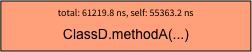
\includegraphics[scale=0.65]{Imagens/no_adicionado.png}
   \textsf{\caption[Nó que representa um método adicionado.]{Nó que representa um método adicionado.\label{fig:no-adicionado}}}
\end{figure}

\begin{itemize}
   \item \textit{Cor}: os nós que foram adicionados na versão atual são mostrados na cor salmão claro;
   \item \textit{Tempos de execução}: os tempos de execução total e do próprio nó são exibidos. No exemplo, o tempo total do nó é de \texttt{61.219,8} nanossegundos e o tempo do próprio nó é de \texttt{55.363,2} nanossegundos.
   %\item \textit{Detalhes}: nos nós adicionados, os detalhes possuem as mesmas informações exibidas para os nós de degradação ou de otimização. No entanto, uma mensagem é exibida em vermelho indicando que o nó adicionado é um potencial causador da degradação de desempenho do cenário. A figura \ref{fig:detalhes-no-adicionado} adiante apresenta esta seção.
\end{itemize}

% \begin{figure}[htb]
%    \centering
%    \frame{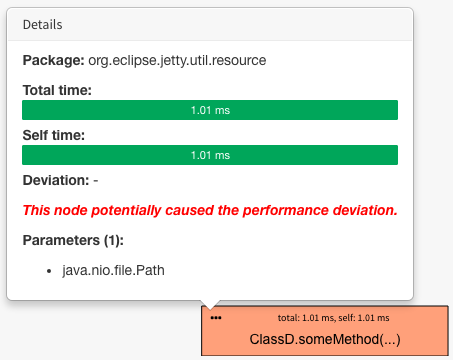
\includegraphics[scale=0.65]{Imagens/detalhes_no_adicionado.png}}
%    \textsf{\caption[Seção de detalhes do nó adicionado.]{Seção de detalhes do nó adicionado.\label{fig:detalhes-no-adicionado}}}
% \end{figure}

\subsubsection{Nó removido} \label{subsec:no-removido}

De maneira contrária ao que foi relatado sobre o nó adicionado, um cenário pode não possuir, na versão atual, chamadas de métodos que estavam presentes na versão anterior. Significa que essas chamadas, para a hierarquia de chamadas de métodos do cenário, foram removidas. No entanto, vale salientar que esse fato não representa que o método em si (código-fonte) foi removido. A figura \ref{fig:no-removido} mostra a representação de um nó removido no grafo. A descrição dos atributos visuais é a que segue:

\begin{figure}[htb]
   \centering
   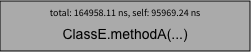
\includegraphics[scale=0.65]{Imagens/no_removido.png}
   \textsf{\caption[Nó que representa um método removido.]{Nó que representa um método removido.\label{fig:no-removido}}}
\end{figure}

\begin{itemize}
   \item \textit{Cor}: os nós que foram removidos na versão atual possuem cor em um tom de cinza;
   \item \textit{Tempos de execução}: os tempos de execução total e do próprio nó na versão anterior são exibidos. No exemplo, o tempo total do nó é de \texttt{164.958,11} nanossegundos e o tempo do próprio nó é de \texttt{95.969,24} nanossegundos.
\end{itemize}

\subsubsection{Nó de agrupamento} \label{subsec:no-agrupamento}

Além dos que representam métodos com ou sem desvio de desempenho, e métodos adicionados e removidos, há um tipo de nó que representa um agrupamento de vários outros: o agrupado. Assim, os que não estão diretamente relacionados com nós de desvio, adicionados ou removidos, são omitidos e representados por um único nó agrupado. A figura \ref{fig:no-agrupamento} a seguir ilustra esse tipo de nó, seguido da descrição dos seus atributos visuais.

\begin{figure}[htb]
   \centering
   \frame{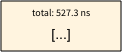
\includegraphics[scale=0.65]{Imagens/no_agrupado.png}}
   \textsf{\caption[Nó que representa um agrupamento de outros nós.]{Nó que representa um agrupamento de outros nós.\label{fig:no-agrupamento}}}
\end{figure}

\begin{itemize}
   \item \textit{Cor}: os nós de agrupamento são mostrados na cor marrom claro;
   \item \textit{Nome do nó}: posicionado ao centro, é exibido o texto \textit{[...]};
   \item \textit{Tempos de execução}: é exibido o tempo de execução total que representa a soma de todos os tempos de execução dos nós contidos no agrupamento. No exemplo, o tempo total é de \texttt{527,3} nanossegundos.
\end{itemize}

Cada nó no grafo de chamadas, da forma como foi apresentado até o momento, representa uma única execução deste. No entanto, um nó, para determinada hierarquia de chamadas, pode ser executado mais de uma vez (por exemplo, em um \textit{loop}). Com o intuito de não acrescentar nós ao grafo para representar essas situações, foi estabelecido que se um nó possuir uma borda espessa, significa que este executou mais de uma vez naquela hierarquia. A figura \ref{fig:no-borda-espessa} adiante exemplifica um nó com uma borda espessa.

\begin{figure}[htb]
   \centering
   \frame{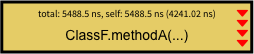
\includegraphics[scale=0.65]{Imagens/no_borda_espessa.png}}
   \textsf{\caption[Borda espessa de um nó, representando múltiplas execuções.]{Borda espessa de um nó, representando múltiplas execuções.\label{fig:no-borda-espessa}}}
\end{figure}

As propriedades visuais apresentadas para a visualização do grafo de chamadas incluem, em suma, três partes: (i) seção de sumário, contendo informações gerais sobre o cenário; (ii) seção de histórico, mostrando o histórico do desempenho do cenário dentre as dez últimas versões analisadas; e (iii) seção do grafo de chamadas, onde a execução dos métodos é representada através de nós e arestas. Esta seção é a mais importante desta visualização, contendo características visuais que diferem os nós de acordo com sua classificação. Um resumo dessas características é apresentado na tabela \ref{tab:resumo-caracteristicas-nos} a seguir.

\begin{table}[!htb]
   \textsf{\caption{Resumo das características visuais dos nós.\label{tab:resumo-caracteristicas-nos}}}
   \centering
   \medskip
   \begin{tabular}{c|c|c|c}
   \textbf{Tipo} & \textbf{Cor}   & \textbf{Tempos de Execução} & \textbf{Setas} \\ \hline
   Sem desvio    & Marrom claro   & Total e próprio         & Sem setas \\ \hline
   Degradado     & Vermelho claro & Total, próprio e desvio & Vermelhas, para baixo \\ \hline
   Otimizado     & Verde claro    & Total, próprio e desvio & Verdes, para cima \\ \hline
   Adicionado    & Salmão claro   & Total e próprio         & Sem setas \\ \hline
   Removido      & Cinza          & Total e próprio         & Sem setas \\ \hline
   Agrupado      & Marrom claro   & Total                   & Sem setas
   \end{tabular}
\end{table}

\subsection{Interação} \label{subsec:interacao-grafo-chamadas}

Esta visualização exibe um conjunto de informações que a torna capaz de indicar os métodos que potencialmente foram responsáveis por desvios de desempenho de um determinado cenário. Contudo, o usuário pode interagir com o grafo efetuando o efeito de zoom, destacando o caminho de execução de determinado nó com desvio ou obtendo mais informações sobre um nó passando o cursor do \textit{mouse} sobre ele.

O zoom pode ser acessado pela barra de ferramentas mostrada na figura \ref{fig:grafo-chamadas-barra-ferramentas}. Essa barra situa-se logo acima da área de desenho do grafo (como pode ser visto na figura \ref{fig:grafo-chamadas-exemplo}) e exibe os botões marcados de \texttt{A} a \texttt{D}. Os botões \texttt{A}, \texttt{B} e \texttt{C} podem ser clicados para realizar o efeito de zoom. O botão A realiza o efeito de distanciamento (\textit{Zoom Out}), o botão B redefine o zoom para o estado inicial (100\%) e o botão C efetua o efeito de aproximação (\textit{Zoom In}). O zoom pode fazer com que o grafo seja comportado novamente na área de desenho.

\begin{figure}[htb]
   \centering
   \frame{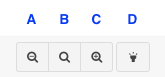
\includegraphics[scale=0.70]{Imagens/grafo_chamadas_barra_ferramentas.png}}
   \textsf{\caption[Barra de ferramentas do grafo de chamadas.]{Barra de ferramentas do grafo de chamadas.\label{fig:grafo-chamadas-barra-ferramentas}}}
\end{figure}

O destaque do caminho de execução de um nó com desvio esmaece todos os nós que não estão no caminho de execução do nó desejado. Existem duas formas de se obter esse efeito: a primeira delas é a partir do botão \texttt{D} da barra de ferramentas. Esse botão, ao ser clicado, destaca os caminhos para todos os nós com desvio mostrados no grafo, como exemplifica a figura \ref{fig:grafo-chamadas-destaque}. Para desfazer o efeito, o botão deve ser clicado novamente; a segunda forma de se obter esse destaque é efetuando um duplo clique em algum dos nós com desvio exibido no grafo. Isso fará com que o caminho do nó raiz até o nó clicado seja destacado, esmaecendo todos os outros. Para reverter o efeito, nessa situação, o usuário pode realizar o duplo clique em qualquer nó sem desvio de desempenho exibido no grafo.

\begin{figure}[htb]
   \centering
   \frame{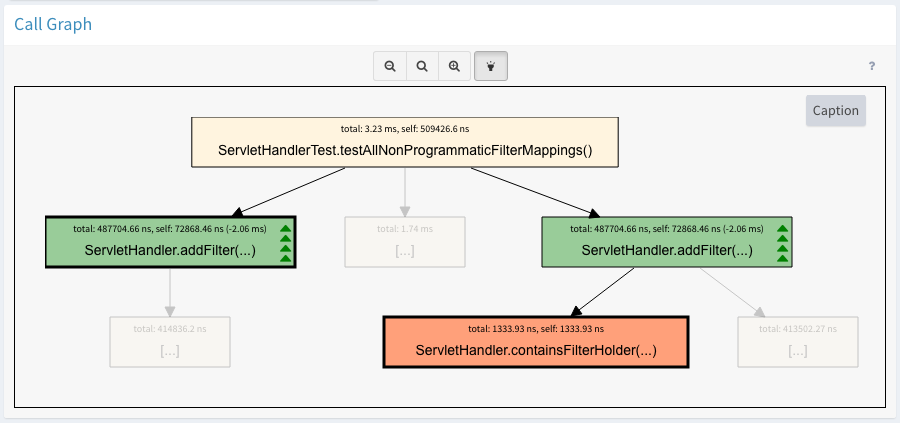
\includegraphics[scale=0.50]{Imagens/grafo_chamadas_destaque.png}}
   \textsf{\caption[Efeito de destaque do caminho de execução de nós com desvio.]{Efeito de destaque do caminho de execução de nós com desvio.\label{fig:grafo-chamadas-destaque}}}
\end{figure}

Uma legenda explicativa também foi implementada para ajudar na interpretação do grafo. O usuário pode acessá-la clicando no botão \texttt{Caption}, no canto superior direito do grafo. Ao ser clicada, a legenda é expandida, exibindo os elementos visuais e seus significados, conforme mostrado na figura \ref{fig:grafo-chamadas-legenda}.

\begin{figure}[htb]
   \centering
   \frame{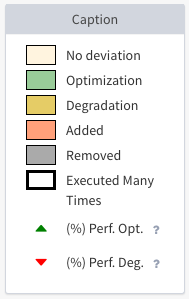
\includegraphics[scale=0.65]{Imagens/grafo_chamadas_legenda.png}}
   \textsf{\caption[Legenda do grafo de chamadas.]{Legenda do grafo de chamadas.\label{fig:grafo-chamadas-legenda}}}
\end{figure}

O usuário pode obter mais detalhes sobre cada nó exibido no grafo. Para isso, ele deve posicionar o ponteiro do mouse sobre o nó desejado e aguardar meio segundo. Após esse tempo, é exibido um \textit{tooltip} com essas informações. A figura \ref{fig:grafo-chamadas-detalhes-no} exemplifica os detalhes de um nó.

\begin{figure}[htb]
   \centering
   \frame{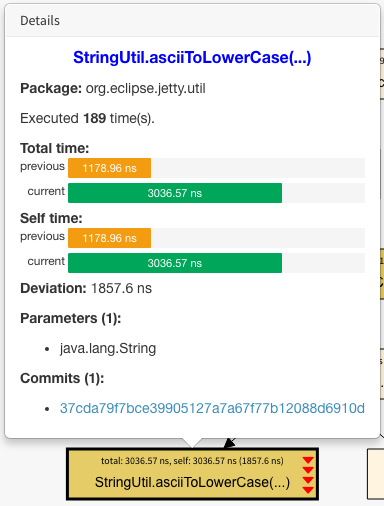
\includegraphics[scale=0.55]{Imagens/grafo_chamadas_detalhes_no.png}}
   \textsf{\caption[Detalhes de um nó no grafo de chamadas.]{Detalhes de um nó no grafo de chamadas.\label{fig:grafo-chamadas-detalhes-no}}}
\end{figure}

Na figura, podem ser encontradas informações sobre o pacote do método representado, a quantidade de vezes que o nó foi executado em caso de execução múltipla, o tempo total na versão anterior e atual, o tempo do próprio nó na versão anterior e atual, o tempo de desvio de desempenho, a listagem de parâmetros do método e a listagem de \textit{commits} que possivelmente causaram o desvio de desempenho do nó. Dependendo do tipo de nó ao qual se quer obter os detalhes, podem existir mais ou menos as informações a serem apresentadas.

\FloatBarrier % evite que as figuras da subsecao anterior invadam a secao seguinte

\subsection{Funcionamento} \label{subsec:funcionamento-visualizacao-2}

Após a execução de uma nova análise, conforme apresentado na seção \ref{subsec:new-analysis}, o funcionamento desta visualização segue o funcionamento geral das visualizações mostrado na figura \ref{fig:funcionamento-geral-visualizacoes}, no entanto, no passo 4 dessa figura, existem processamentos específicos a fim de tratar os dados antes de serem exibidos para o usuário.

Seguindo o fluxo da figura \ref{fig:funcionamento-geral-visualizacoes}, a partir da visualização de sumarização de cenários, o usuário pode clicar em uma das fatias daquele gráfico e realizar uma requisição para a visualização do grafo de chamadas (passo 1). O servidor recebe essa requisição e, a partir dos parâmetros enviados, recupera do banco de dados QAV (passo 2) os dados necessários para a visualização. Após isso, é retornado para o navegador do usuário um arquivo em formato JSON contendo os dados recuperados (passo 3). O navegador, por fim, recebe, interpreta esse arquivo e monta a visualização com as devidas informações para que a renderização seja feita com sucesso (passo 4).

No passo 4 da figura \ref{fig:funcionamento-geral-visualizacoes}, há um procedimento executado no navegador do usuário que recebe e processa o arquivo JSON e, ao final, renderiza o grafo de chamadas. Esse processo está exposto em detalhes na figura \ref{fig:grafo-chamadas-passo-4} adiante. O início ocorre ao receber o arquivo do servidor e a primeira atividade é criar a área de desenho que abrigará o grafo. Nessa atividade são considerados a altura e largura do monitor do usuário, de modo que a área útil de apresentação seja compatível com a área do monitor.

\begin{figure}[!htb]
   \centering
   \frame{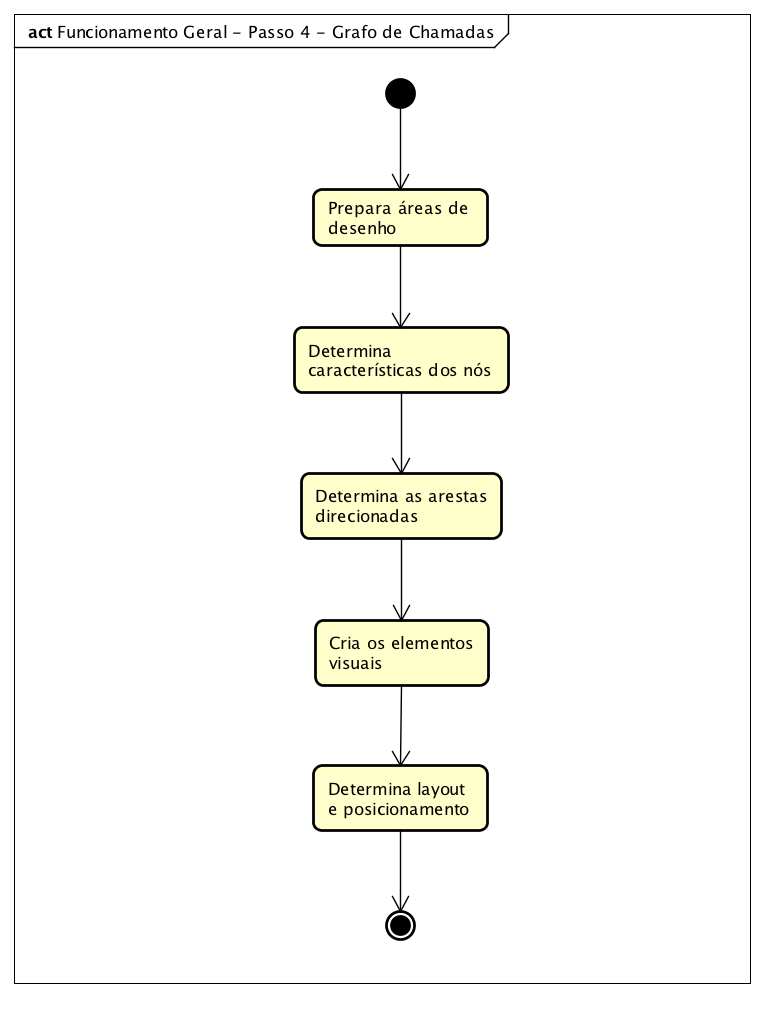
\includegraphics[scale=0.50]{Imagens/grafo_chamadas_passo_4.png}}
   \textsf{\caption[Detalhamento do passo 4 da figura \ref{fig:funcionamento-geral-visualizacoes}, no Grafo de Chamadas.]{Detalhamento do passo 4 da figura \ref{fig:funcionamento-geral-visualizacoes}, no Grafo de Chamadas.\label{fig:grafo-chamadas-passo-4}}}
\end{figure}

Após isso, as características dos nós contidos no arquivo JSON são determinadas. Para cada um deles, são determinados: (i) a altura e largura da sua caixa, que é diretamente proporcional ao tamanho do nome a ser exibido. Vale salientar que o pacote da classe é omitido para a exibição do nome; (ii) a espessura da borda, caso o nó tenha sido executado mais de uma vez; (iii) a cor, que depende do seu tipo; (iv) os tempos de execução total e, caso pertinente, o do próprio nó e o de desvio; (v) as setas, que dependem do seu tipo e da porcentagem de desvio do tempo de execução ocorrida de uma versão para outra; e (vi) os detalhes a serem exibidos no \textit{tooltip}, que dependem do tipo do nó.

Depois, as arestas são determinadas de acordo com a relação de nós pais e filhos contidos no arquivo. Elas são direcionadas do nó pai para os filhos, indicando a hierarquia de chamadas.

Com a definição dos nós e suas características, e das arestas, a próxima atividade do processo é criar os elementos visuais na área de desenho, para, posteriormente, determinar o \textit{layout} (conforme citado anteriormente, o \textit{layout} utilizado é em árvore) e posicionamento dos nós. Por fim, o grafo de chamadas é renderizado para o usuário.

\subsection{Exemplo de Uso da Ferramenta: Jetty {\color{red}fica ou sai?}} \label{subsec:exemplo-uso-jetty}

Foi realizado um estudo de caso para exemplificar o uso das visualizações. Para tanto, foi utilizado duas versões da aplicação Jetty \cite{Jetty2016}: 9.2.6 e 9.3.0.M1. Esse sistema faz parte do Projeto Eclipse e é um \textit{framework open-source} que provê um servidor web além de um servlet container Java. Essa aplicação foi escolhida para o estudo de caso pois todos os tipos de nós foram capazes de ser exemplificados.

Para a primeira fase do \textit{\perfMinerName}, a análise dinâmica, todos os testes automatizados foram considerados cenários. Como os testes são implementados em JUnit 4, o aspecto interceptou todos os métodos marcados com a anotação \texttt{@Test} como métodos de entrada de um cenário. A análise dinâmica, como mencionado anteriormente, foi executada no mesmo computador para ambas as versões, nas mesmas condições e com todos os serviços não essenciais desabilitados. A suíte de testes do Jetty foi executada 30 vezes para que as medições de desempenho fossem mais precisas em termos de tempo de execução \cite{Pinto2015}.

A resultado da análise foi um total de 11 cenários, sendo 7 com degradação do desempenho e 4 com otimização. No grafo gerado, é possível que dois nós representem o mesmo método, indicando duas execuções, e as arestas direcionadas representam invocações entre os métodos. A figura \ref{fig:exemplo-degradacao} exemplifica o grafo de um cenário com degradação.

\begin{figure}[!htb]
   \centering
   \frame{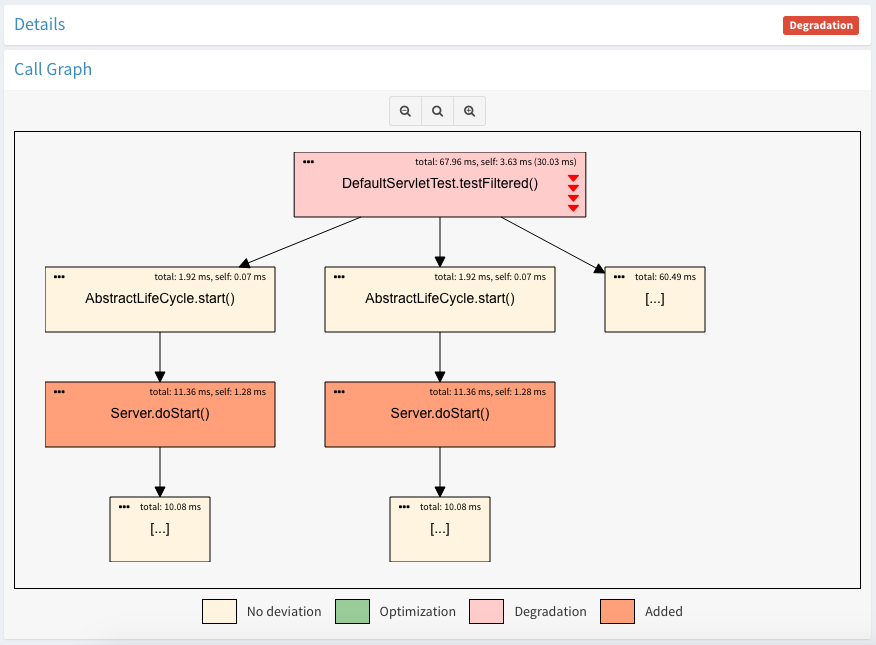
\includegraphics[scale=0.52]{Imagens/exemplo_degradacao.png}}
   \textsf{\caption[Grafo de chamadas de um cenário com degradação de desempenho.]{Grafo de chamadas de um cenário com degradação de desempenho.\label{fig:exemplo-degradacao}}}
\end{figure}

O grafo exibido destaca que o nó raiz, \texttt{DefaultServletTest.testFiltered()}, teve uma degradação de desempenho de mais de 75\%, indicado pela cor do nó, laranja amarelo, e pelas quatro setas vermelhas para baixo. É possível notar também que dois nós que representam o método \texttt{Server.doStart()} foram adicionados. Isso significa que durante a execução do cenário \texttt{Entry point for DefaultServletTest.testFiltered} duas chamadas a esse método foram efetuadas na versão 9.3.0.M1, e elas não existiam na versão 9.3.6. Os nós adicionados são indicados como potenciais causadores de degradação de desempenho, de modo que, possivelmente, esses nós influenciaram na degradação do raiz. Na visualização há nós que não têm relação com os desvios, representados como agrupados, e nós sem desvio, representados na cor marrom claro.

Na mesma figura, além do próprio grafo, na parte superior da seção \textit{Call Graph} é encontrada uma barra de ferramentas com botões de \textit{Zoom Out}, \textit{Zoom to Fit} e \textit{Zoom In}; e na parte inferior é exibida uma legenda ajudando os usuários a identificarem os nós do grafo. Os botões de \textit{zoom} e a legenda são exibidos para todos os grafos, independente da quantidade de nós ou do tipo de desvio ocorrido.

Na figura \ref{fig:exemplo-detalhes-degradacao} adiante, a seção \textit{Details} desse cenário é exibida expandida, indicando, no rótulo, que o cenário teve o seu desempenho degradado entre as versões, e que o total de nós para esse cenário foi de 1695.

\begin{figure}[!htb]
   \centering
   \frame{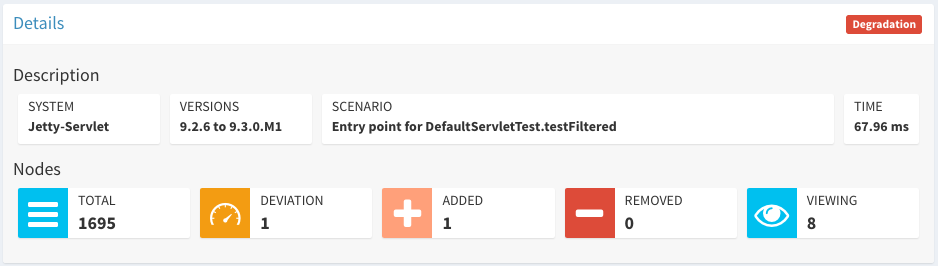
\includegraphics[scale=0.48]{Imagens/exemplo_detalhes_degradacao.png}}
   \textsf{\caption[Detalhes de um cenário com degradação de desempenho.]{Detalhes de um cenário com degradação de desempenho.\label{fig:exemplo-detalhes-degradacao}}}
\end{figure}

A figura \ref{fig:exemplo-otimizacao} a seguir apresenta o cenário \texttt{Entry point for ServletContextHandler\\Test.testFallThrough} com otimização de desempenho. Dois nós contribuíram para esse desvio, identificados pela cor verde claro: \texttt{Server.doStart()} e \texttt{ServletContextHandler.\\relinkHandlers()}. No primeiro, a variação foi entre 50\% e 75\%, ao passo que no segundo foi de mais de 75\%. Há ainda a representação de nós agrupados e sem desvio.

\begin{figure}[!htb]
   \centering
   \frame{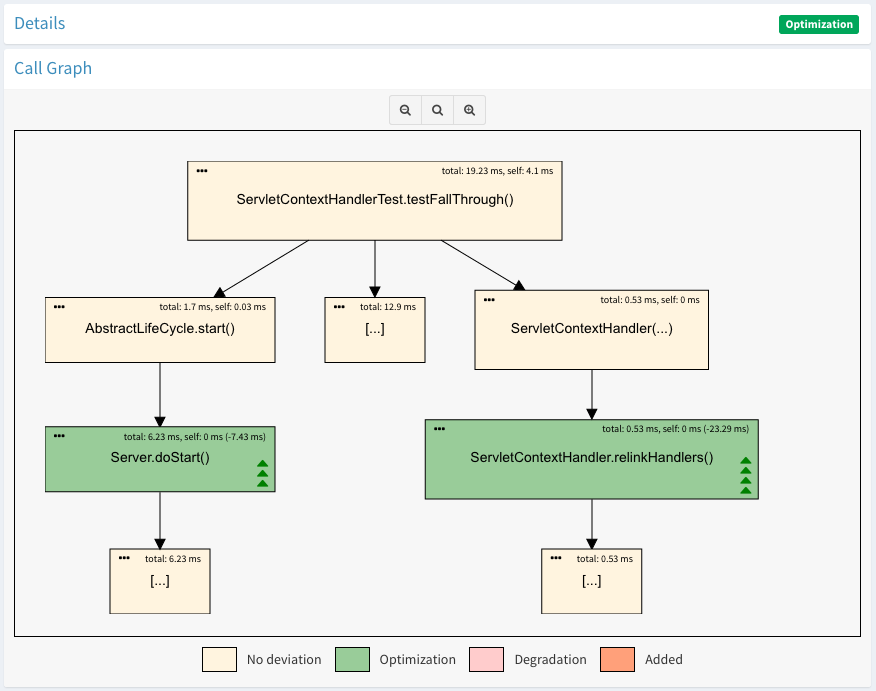
\includegraphics[scale=0.52]{Imagens/exemplo_otimizacao.png}}
   \textsf{\caption[Grafo de chamadas de um cenário com otimização de desempenho.]{Grafo de chamadas de um cenário com otimização de desempenho.\label{fig:exemplo-otimizacao}}}
\end{figure}

\begin{figure}[!htb]
   \centering
   \frame{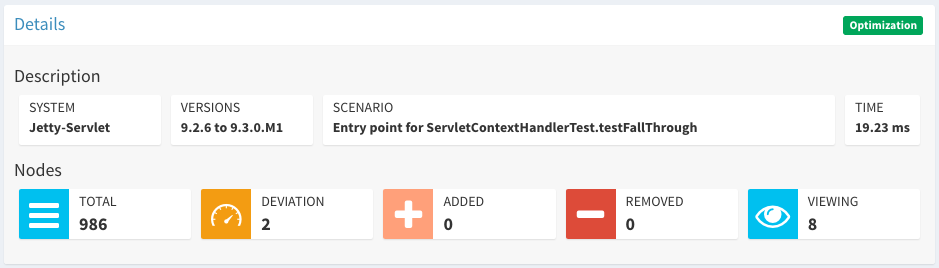
\includegraphics[scale=0.48]{Imagens/exemplo_detalhes_otimizacao.png}}
   \textsf{\caption[Detalhes de um cenário com otimização de desempenho.]{Detalhes de um cenário com otimização de desempenho.\label{fig:exemplo-detalhes-otimizacao}}}
\end{figure}

A seção \textit{Details} expandida pode ser vista na figura \ref{fig:exemplo-detalhes-otimizacao}. O rótulo de otimização é exibido no canto superior esquerdo indicando o tipo de desvio ocorrido no cenário. A figura indica um total de 986 nós para esse cenário.

% A tabela \ref{tab:jetty-v9.2.6-v9.3.0.M1} a seguir mostra uma lista com todos os cenários para o sistema Jetty, versões 9.2.6 para 9.3.0.M1. Nela, são exibidas as porcentagens de desvio de degradação ou otimização para os cenários.

% \begin{sidewaystable}[!htb]
%    \textsf{\caption{Cenários para o Jetty, versões 9.2.6 para 9.3.0.M1.\label{tab:jetty-v9.2.6-v9.3.0.M1}}}
%    \centering
%    \medskip
%    \begin{tabular}{l|c|c|c|c}
%    \multicolumn{1}{c|}{\textbf{Nome}}                                                                                                       & \textbf{\begin{tabular}[c]{@{}c@{}}Tempo \\ v9.2.6 (ms)\end{tabular}} & \textbf{\begin{tabular}[c]{@{}c@{}}Tempo \\ v9.3.0.M1 (ms)\end{tabular}} & \textbf{\begin{tabular}[c]{@{}c@{}}Variação \\ (\%)\end{tabular}} & \textbf{\begin{tabular}[c]{@{}c@{}}Tipo de \\ Desvio\end{tabular}} \\ \hline
%    \begin{tabular}[c]{@{}l@{}}Entry point for \\ DispatcherForwardTest.testQueryRetainedByForward\\ WithoutQuery\end{tabular}              & 569,26                                                                & 597,33                                                                   & 4,93                                                              & Degradação                                                         \\ \hline
%    \begin{tabular}[c]{@{}l@{}}Entry point for \\ SSLAsyncIOServletTest.testAsyncIOWritesWith\\ Aggregation\end{tabular}                    & 549,21                                                                & 587,55                                                                   & 6,98                                                              & Degradação                                                         \\ \hline
%    \begin{tabular}[c]{@{}l@{}}Entry point for \\ AsyncServletLongPollTest.testSuspendedRequest\\ CompletedByAnotherRequest\end{tabular}    & 620,36                                                                & 634,60                                                                   & 2,29                                                              & Degradação                                                         \\ \hline
%    Entry point for DefaultServletTest.testFiltered                                                                                         & 37,93                                                                 & 67,96                                                                    & 79,17                                                             & Degradação                                                         \\ \hline
%    \begin{tabular}[c]{@{}l@{}}Entry point for \\ ServletContextHandlerTest.testReplaceServlet\\ HandlerWithoutServlet\end{tabular}         & 429,60                                                                & 453,96                                                                   & 5,67                                                              & Degradação                                                         \\ \hline
%    \begin{tabular}[c]{@{}l@{}}Entry point for \\ AsyncContextListenersTest.testAsyncDispatch\\ AsyncCompletePreservesListener\end{tabular} & 601,83                                                                & 622,96                                                                   & 3,51                                                              & Degradação                                                         \\ \hline
%    \begin{tabular}[c]{@{}l@{}}Entry point for \\ AsyncIOServletTest.testAsyncWriteThrowsError\end{tabular}                                 & 599,10                                                                & 611,00                                                                   & 1,98                                                              & Degradação                                                         \\ \hline
%    \begin{tabular}[c]{@{}l@{}}Entry point for \\ DispatcherForwardTest.testQueryAggregatesWith\\ FormByForwardWithoutQuery\end{tabular}    & 26,46                                                                 & 20,76                                                                    & 21,54                                                             & Otimização                                                         \\ \hline
%    \begin{tabular}[c]{@{}l@{}}Entry point for \\ ServletContextHandlerTest.testFallThrough\end{tabular}                                    & 52,00                                                                 & 19,23                                                                    & 63,01                                                             & Otimização                                                         \\ \hline
%    \begin{tabular}[c]{@{}l@{}}Entry point for \\ AsyncContextListenersTest.testListenerCleared\\ OnSecondRequest\end{tabular}              & 23,90                                                                 & 17,16                                                                    & 28,20                                                             & Otimização                                                         \\ \hline
%    \begin{tabular}[c]{@{}l@{}}Entry point for \\ ServletContextHandlerTest.testAddServletAfterStart\end{tabular}                           & 55,56                                                                 & 20,40                                                                    & 63,28                                                             & Otimização                                                     
%    \end{tabular}
% \end{sidewaystable}

%A maior variação absoluta foi para o cenário \texttt{Entry point for DefaultServletTest\\.testFiltered}, uma degradação de 79,17\%. Como destacado na figura \ref{fig:exemplo-degradacao}, dois nós com tempos significantes com relação ao cenário foram adicionados, provavelmente, causando a degradação. O gráfico \ref{fig:grafico-jetty-v9.2.6-v9.3.0.M1} adiante exibe a porcentagem de variação de desempenho.

% \begin{sidewaysfigure}[!htb]
%    \centering
%    \frame{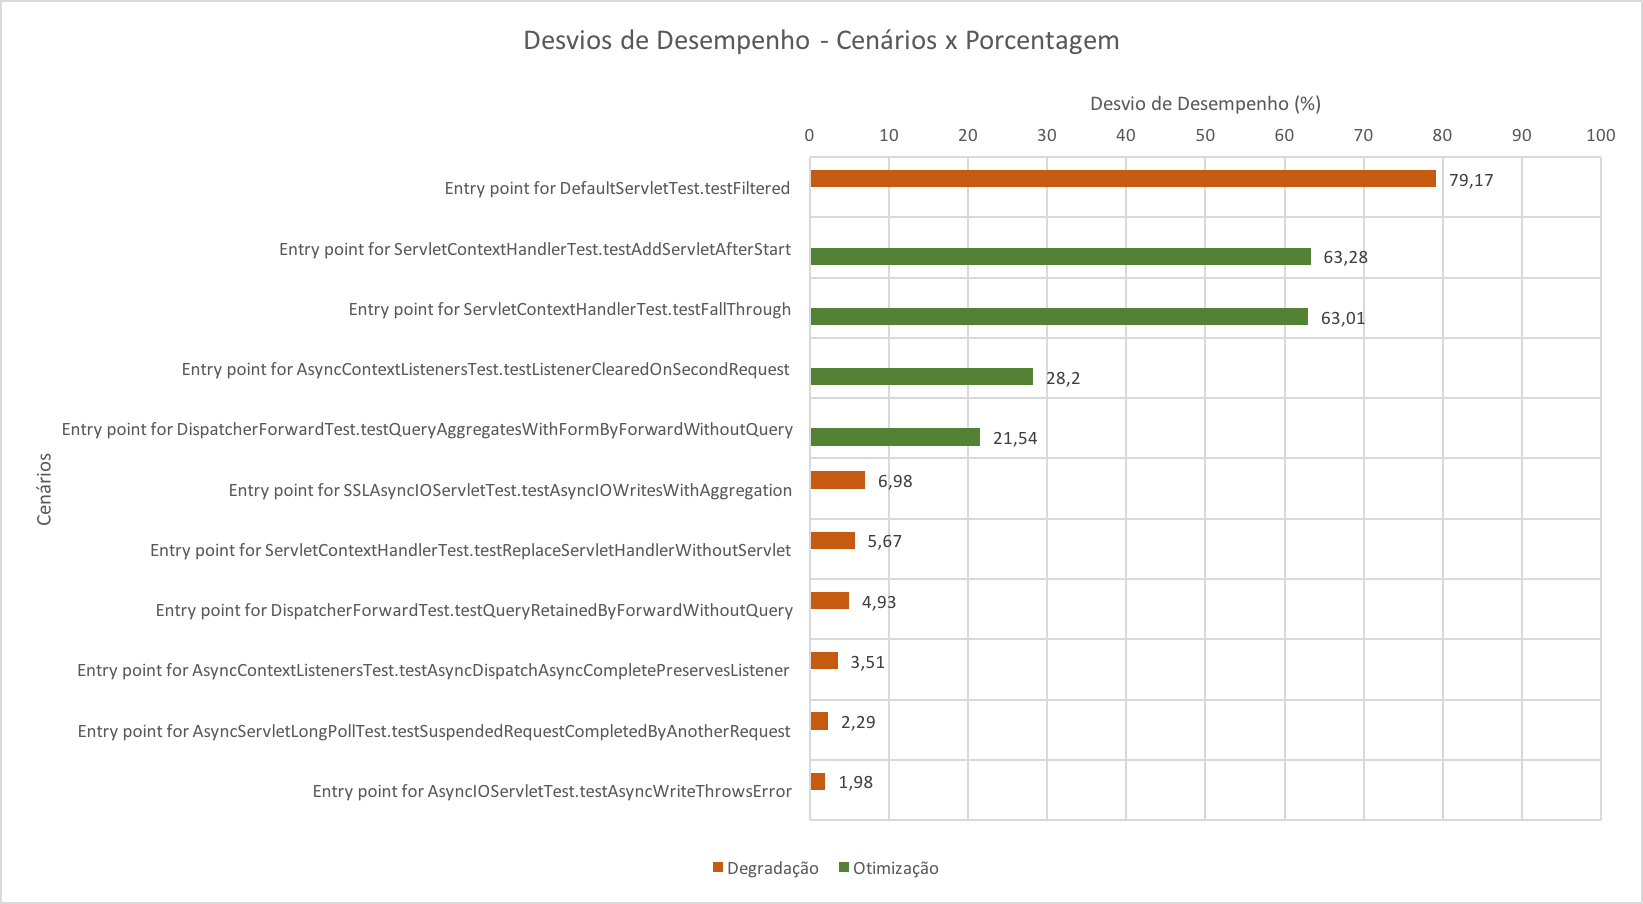
\includegraphics[scale=0.80]{Imagens/grafico_jetty_v926_v931M1.png}}
%    \textsf{\caption[Porcentagem de desvios de desempenho para o Jetty, versões 9.2.6 para 9.3.0.M1.]{Porcentagem de desvios de desempenho para o Jetty, versões 9.2.6 para 9.3.0.M1.\label{fig:grafico-jetty-v9.2.6-v9.3.0.M1}}}
% \end{sidewaysfigure}

\section{Considerações} \label{sec:consideracoes-cap3}

Um dos principais desafios do processo de manutenção de um software é compreendê-lo adequadamente, em especial, a sua arquitetura. A falta de acompanhamento da evolução da arquitetura ao longo do tempo pode levar a sua degradação, impactando os seus atributos de qualidade. Este capítulo apresentou visualizações de arquitetura de software que visam tornar direta e fácil a monitoração da evolução arquitetural, com relação ao atributo de qualidade de desempenho. Uma vez que as ferramentas existentes se mostram complexas ou ineficientes para essa finalidade, as visualizações foram propostas a serem implementadas como extensões da ferramenta \textit{\perfMinerName}. Em suma, são as seguintes:
\begin{enumerate}[(i)]
   \item \textit{Sumarização dos Cenários}: a sumarização dos cenários com desvio de desempenho objetiva mostrar, de maneira sucinta, quais cenários analisados tiveram desvio de desempenho, seja degradação ou otimização;
   \item \textit{Grafo de Chamadas}: a visualização do grafo de chamadas exibe, para cada cenário, as chamadas dos métodos que tiveram desvio de desempenho. Dessa forma, o usuário pode localizar em qual trecho de código da execução do cenário houve o desvio.
\end{enumerate}

A visualização da sumarização de cenários permite aos usuários ter uma visão geral de todos os cenários indicados com desvios de desempenho entre uma determinada versão e a anterior. A visualização mostra os cenários em um gráfico de rosca, onde cada cenário é representado por uma fatia dessa rosca, e todos os cenários compõem a integralidade do gráfico. Dessa forma, os usuários podem identificar se os cenários exibidos são de degradação ou otimização, identificar o cenário com maior tempo de execução dentre os exibidos e o que possuiu a maior porcentagem de desvio de desempenho.

Foi mostrado os detalhes da visualização do grafo de chamadas, que visa exibir, para dadas duas versões de um sistema, os métodos que potencialmente causaram o desvio de desempenho para um determinado cenário. Nesta visualização, os métodos são apresentados em um grafo direcionado de chamadas com propriedades visuais que destacam quais dos métodos mostrados tiveram desvios de desempenho. Com essa visualização, os usuários podem identificar as possíveis causas de desvios de desempenho em determinado cenário através da listagem de \textit{commits} presentes em cada nó com desvio de desempenho, adicionado ou removido.